\title{SNSにおいてフェイクニュースを拡散するユーザの特徴抽出}
\author{プロジェクトマネジメントコース\\
ソフトウェア開発管理グループ\\
矢吹研究室\\
1442014\\
岩橋瑠伊}
\date{}
\begin{document}
\maketitle

%本テンプレートの余白は,卒論マニュアルで指示されたものとは違っているが,1ページあたりの文字数は40文字x40行と,卒論マニュアル通りになっている。文字間隔や行間隔を調整して,余白をマニュアル通りにすることもできるが,それでは文章が読みにくくなるため,このような対応をしている。

%\noindent
□□□□□□□□□■□□□□□□□□□■□□□□□□□□□■□□□□□□□□□■
□□□□□□□□□■□□□□□□□□□■□□□□□□□□□■□□□□□□□□□■
□□□□□□□□□■□□□□□□□□□■□□□□□□□□□■□□□□□□□□□■
□□□□□□□□□■□□□□□□□□□■□□□□□□□□□■□□□□□□□□□■
□□□□□□□□□■□□□□□□□□□■□□□□□□□□□■□□□□□□□□□■
□□□□□□□□□■□□□□□□□□□■□□□□□□□□□■□□□□□□□□□■
□□□□□□□□□■□□□□□□□□□■□□□□□□□□□■□□□□□□□□□■
□□□□□□□□□■□□□□□□□□□■□□□□□□□□□■□□□□□□□□□■
□□□□□□□□□■□□□□□□□□□■□□□□□□□□□■□□□□□□□□□■
□□□□□□□□□■□□□□□□□□□■□□□□□□□□□■□□□□□□□□□■
□□□□□□□□□■□□□□□□□□□■□□□□□□□□□■□□□□□□□□□■
□□□□□□□□□■□□□□□□□□□■□□□□□□□□□■□□□□□□□□□■
□□□□□□□□□■□□□□□□□□□■□□□□□□□□□■□□□□□□□□□■
□□□□□□□□□■□□□□□□□□□■□□□□□□□□□■□□□□□□□□□■
□□□□□□□□□■□□□□□□□□□■□□□□□□□□□■□□□□□□□□□■
□□□□□□□□□■□□□□□□□□□■□□□□□□□□□■□□□□□□□□□■
□□□□□□□□□■□□□□□□□□□■□□□□□□□□□■□□□□□□□□□■
□□□□□□□□□■□□□□□□□□□■□□□□□□□□□■□□□□□□□□□■
□□□□□□□□□■□□□□□□□□□■□□□□□□□□□■□□□□□□□□□■
□□□□□□□□□■□□□□□□□□□■□□□□□□□□□■□□□□□□□□□■
□□□□□□□□□■□□□□□□□□□■□□□□□□□□□■□□□□□□□□□■
□□□□□□□□□■□□□□□□□□□■□□□□□□□□□■□□□□□□□□□■
□□□□□□□□□■□□□□□□□□□■□□□□□□□□□■□□□□□□□□□■
□□□□□□□□□■□□□□□□□□□■□□□□□□□□□■□□□□□□□□□■
□□□□□□□□□■□□□□□□□□□■□□□□□□□□□■□□□□□□□□□■
□□□□□□□□□■□□□□□□□□□■□□□□□□□□□■□□□□□□□□□■
□□□□□□□□□■□□□□□□□□□■□□□□□□□□□■□□□□□□□□□■
□□□□□□□□□■□□□□□□□□□■□□□□□□□□□■□□□□□□□□□■
□□□□□□□□□■□□□□□□□□□■□□□□□□□□□■□□□□□□□□□■
□□□□□□□□□■□□□□□□□□□■□□□□□□□□□■□□□□□□□□□■
□□□□□□□□□■□□□□□□□□□■□□□□□□□□□■□□□□□□□□□■
□□□□□□□□□■□□□□□□□□□■□□□□□□□□□■□□□□□□□□□■
□□□□□□□□□■□□□□□□□□□■□□□□□□□□□■□□□□□□□□□■
□□□□□□□□□■□□□□□□□□□■□□□□□□□□□■□□□□□□□□□■
□□□□□□□□□■□□□□□□□□□■□□□□□□□□□■□□□□□□□□□■
□□□□□□□□□■□□□□□□□□□■□□□□□□□□□■□□□□□□□□□■
□□□□□□□□□■□□□□□□□□□■□□□□□□□□□■□□□□□□□□□■
□□□□□□□□□■□□□□□□□□□■□□□□□□□□□■□□□□□□□□□■
□□□□□□□□□■□□□□□□□□□■□□□□□□□□□■□□□□□□□□□■
■■■■■■■■■■■■■■■■■■■■■■■■■■■■■■■■■■■■■■■■
□□□□□□□□□■□□□□□□□□□■□□□□□□□□□■□□□□□□□□□■%文字数チェック用

\tableofcontents%目次

\chapter{序論}
Twitterには日常的なことからニュースまで,様々な情報が流れている.本研究では,その中でもデマツイートという嘘の情報に絞って分析を行う.

\chapter{背景}

\section{デマツイートの影響}
SNS上でフェイクニュースを拡散するユーザの特徴について調査する.SNSなどのウェブ上のメディアで,フェイクニュースが問題視されている\cite{dema1}.

例えば,2011年3月11日に発生した東日本大震災時に,携帯電話がつながらない状況下での有用な連絡手段として活躍した.しかし,その有用性はデマや誤情報も大量に拡散させる手助けとなりえる.実際に東日本大震災時に,数十種類のデマや誤情報が情報として拡散されてしまい,日本中を混乱させた.震災時のように連絡手段が限られた状況はこれからも発生する可能性は十分にあり,対策が必要である\cite{dema2}.

\section{デマを拡散するユーザー}
本研究では,デマが拡散されることを防ぐためにデマツイートをリツイートしているユーザの特徴抽出を行う.デマツイートがリツイートされる原因として,デマをデマと見抜けないユーザ,面白半分でリツイートしているユーザの2種類がいると考えた.この2種類のユーザと,それ以外のユーザにはTwitterの使い方に違いがあるのではないかと考えた.

\chapter{目的}
デマツイートをリツイートするユーザーと,それ以外のユーザーのTwitterの使い方に違いを見つける.違いからデマツイートをリツイートするユーザーなのかを判別できるようにする.

\chapter{Twitterについて}

\section{本章の構成}
本章では本研究で使用するTwitterについて説明する.

\section{Twitterとは}
Twitterは,「ツイート」と称される140文字以内の短文の投稿を共有するウェブ上の情報サービスである.
\begin{figure}[h]
\centering
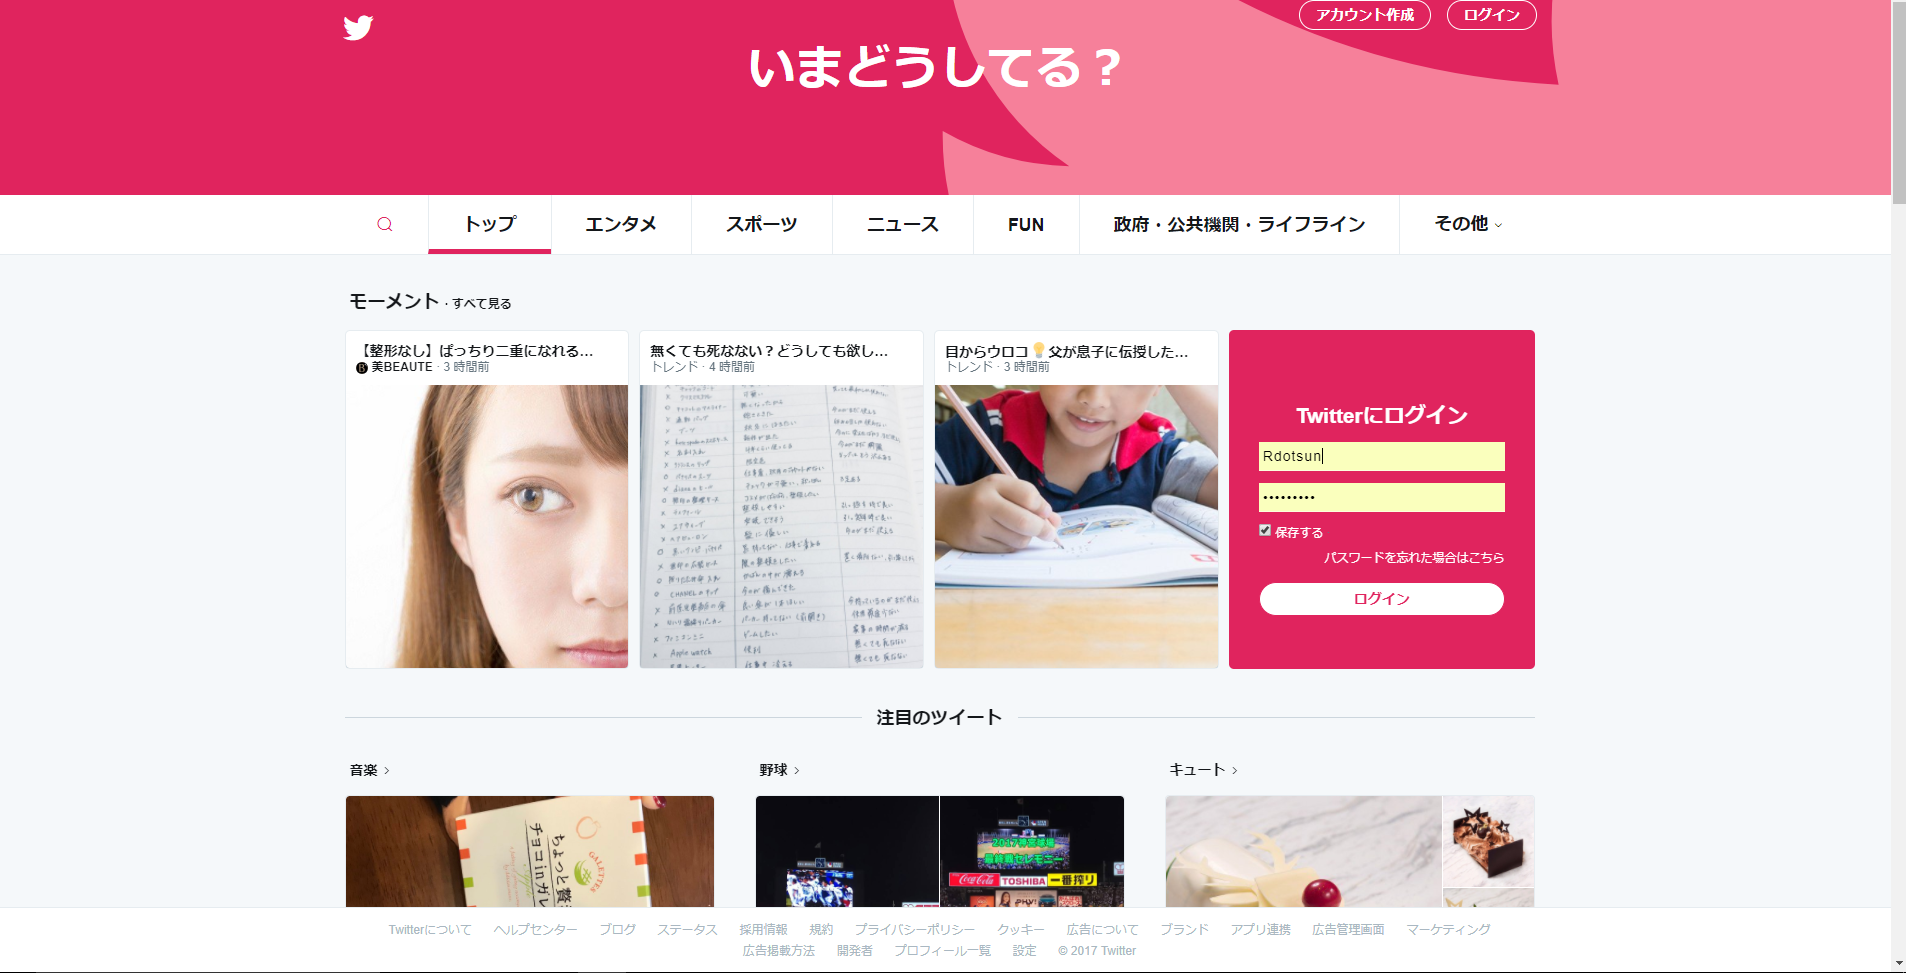
\includegraphics[width=13cm]{01.png}
\caption{Twitterホームページ}\label{1}
\end{figure}
\clearpage

\section{用語}
本節では,Twitterの用語について説明する.

\subsection{ツイート}
140文字以下の文字列のこと.つぶやきとも呼ばれる.
\begin{figure}[htb]
\centering
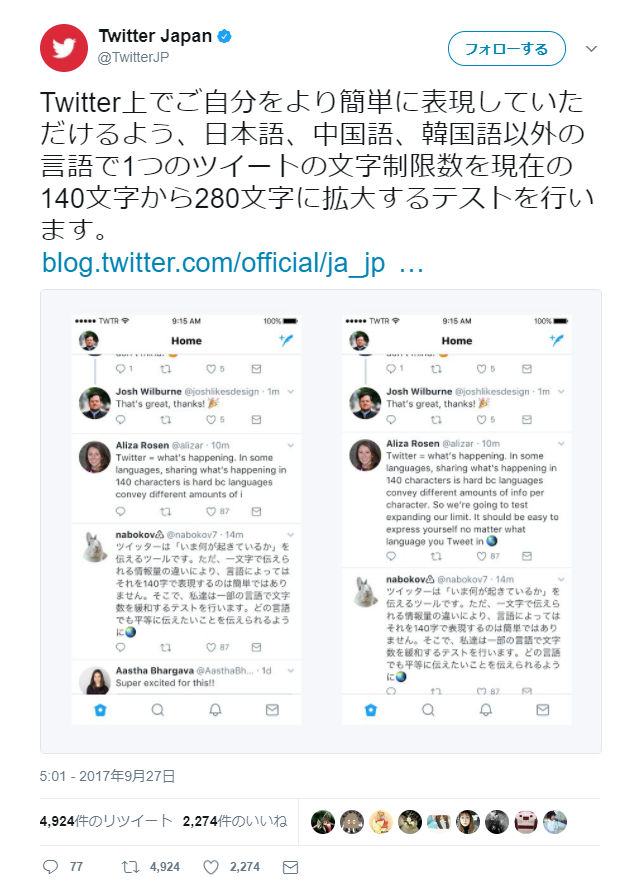
\includegraphics[width=10cm]{02.png}
\caption{ツイートの例}\label{2}
\end{figure}
\clearpage

\subsection{ユーザー}
Twitterを利用している者を指す.
 
\subsection{ユーザー名}
半角英数字,アンダーバーから計15文字以内で作るユーザーの名前である.

\subsection{タイムライン}
ユーザー自身のホーム画面のことである.フォローしているユーザーのつぶやきや,自身のつぶやき,リツイートされたツイートなどの情報が羅列されていく.
\begin{figure}[htb]
\centering
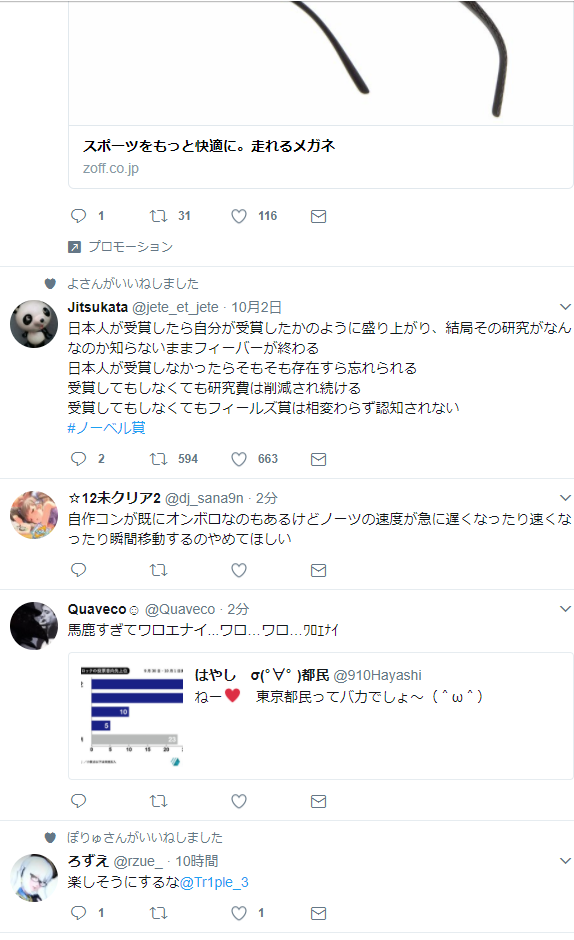
\includegraphics[width=10cm]{03.png}
\caption{タイムラインの例}\label{3}
\end{figure}
\clearpage

\subsection{フォロー}
他人のツイートを購読する機能のこと.他人を「フォロー」することで,その人のツイートがTLに表示されるようになる.フォローは基本的に一方的に行われ,許可の必要はなくフォローし返さなければならないということもない.

\subsection{フォロワー}
自分をフォローしているユーザーのこと.フォロワーのタイムラインに自分(フォローされている人)のつぶやきが表示される.

\subsection{リムーブ}
フォローを解除すること.

\subsection{ブロック}
迷惑なユーザーや嫌いなユーザーなどを遮断する機能のこと.他人をブロックした場合,そのユーザーからのフォローを遮断しそのユーザーのツイートがRTされても自分のTLには表示されなくなる.

\subsection{リツイート}
他の人のツイートを再びツイートすること.自分のタイムラインに流れてきたツイートをリツイートすると,自分のフォロワーのタイムラインにそのツイートが流れる.逆に自分がフォローしているユーザーがリツイートすると,自分のタイムラインにそのツイートが流れる.

\subsection{リプライ}
特定のユーザー名(@...) から始まるツイートをリプライという.そのユーザー宛のツイートということになる.リプライを送った側と,送られた側の両方をフォローしているユーザーのタイムラインには表示されるが,片方のみをフォローしている第三者のタイムラインには表示されない.

\subsection{いいね}
あとで読み返したいと思ったツイートや気に入ったツイートを,♡マークを付けて自分のいいねリストへ登録すること.以前はお気に入り (Favorites) だったが,2015年11月4日,「いいね」に変更され,これまでの「☆」から「♡」に変更された.

\subsection{メンション}
「@ユーザー名」を含むツイートの一覧.

\chapter{TwitterAPIについて}

\section{本章の構成}
本章では本研究で使用するTwitterAPIについて説明する.

\section{TwitterAPIとは}
Twitter社が提供しているサービスで,WebサイトやアプリなどからTwitterの機能を呼び出すことができる.このAPIを利用することでツイートの参照や検索などを行なえるアプリケーション開発ができるようになる.

\subsection{API}
アプリケーションプログラムインターフェイス(Application Program Interface)の略で,プログラミングの際に使用できる命令や規約,関数等の集合のことを示す.ソフトウェア開発の際,いちから全てを作るより,APIを利用すればもともとあるプログラムを呼び出して,その機能を組み込んだソフトウェアを開発することができる.

\subsection{Twitter API}
Twitter社が提供するサービス.WebサイトやアプリケーションなどからTwitterの機能を呼び出すことができ,ツイートの参照や検索等を行えるアプリケーション開発を行えるようになる.

\subsection{REST API}
Twitter APIのパラメータ(リソース)を指定し,特定のURLにHTTPでアクセスすると,JSON形式で記述されたメッセージがレスポンスされるシステム.これはツイートの更新や参照を行う際に使用する基本的なAPIとなる.ただし利用制限があり,15分以内に同じ機能を特定の回数利用すると,はじめにその機能を利用した時間から15分経過するまではその機能が利用できなくなる.

\subsection{Streaming API}
タイムラインの変更をリアルタイムで自動に受け取ることができる.

\subsection{Access Token}
Webサービスを利用するために,認証局がユーザーを認証するために払い出した認証情報のことを指す.ここで言う認証局とはユーザーを認証する情報を保持しており,ユーザーを認証することができるWebサーバーで,Webサービスを提供しているWebサーバー,または,ユーザーを認証することができる第三者のWebサーバーなどを示す.

\chapter{開発環境構築ツールの解説}

\section{本章の構成}
本章では本研究で使用する開発環境構築ツールについて説明する.

\section{Chocolateyとは}
「Chocolatey」は,コマンドラインによるアプリケーションの導入や削除を実現するパッケージ管理システム.パッケージ管理システムとは,アプリケーションやコンポーネント,ライブラリなどの管理を円滑に行うための仕組み.アプリケーションやライブラリを構成するファイル群を1つの”パッケージ”ファイルにまとめ,それを”リポジトリ”へ保管し,コマンドで取得・セットアップを行う.動作に必要な外部コンポーネントがあれば,その導入も自動で行われるのが一般的で,アプリケーションのインストールやアンインストールの手間を省くことができる.Linuxディストリビューションの多くは”apt-get”や”yum”といったパッケージ管理のためのコマンドを備えており,コマンドを入力するだけで手軽にソフトをダウンロード・インストール・アンインストールできて非常に便利.「Chocolatey」はこれをWindows環境で実現しようというものである.
\begin{figure}[htb]
\centering
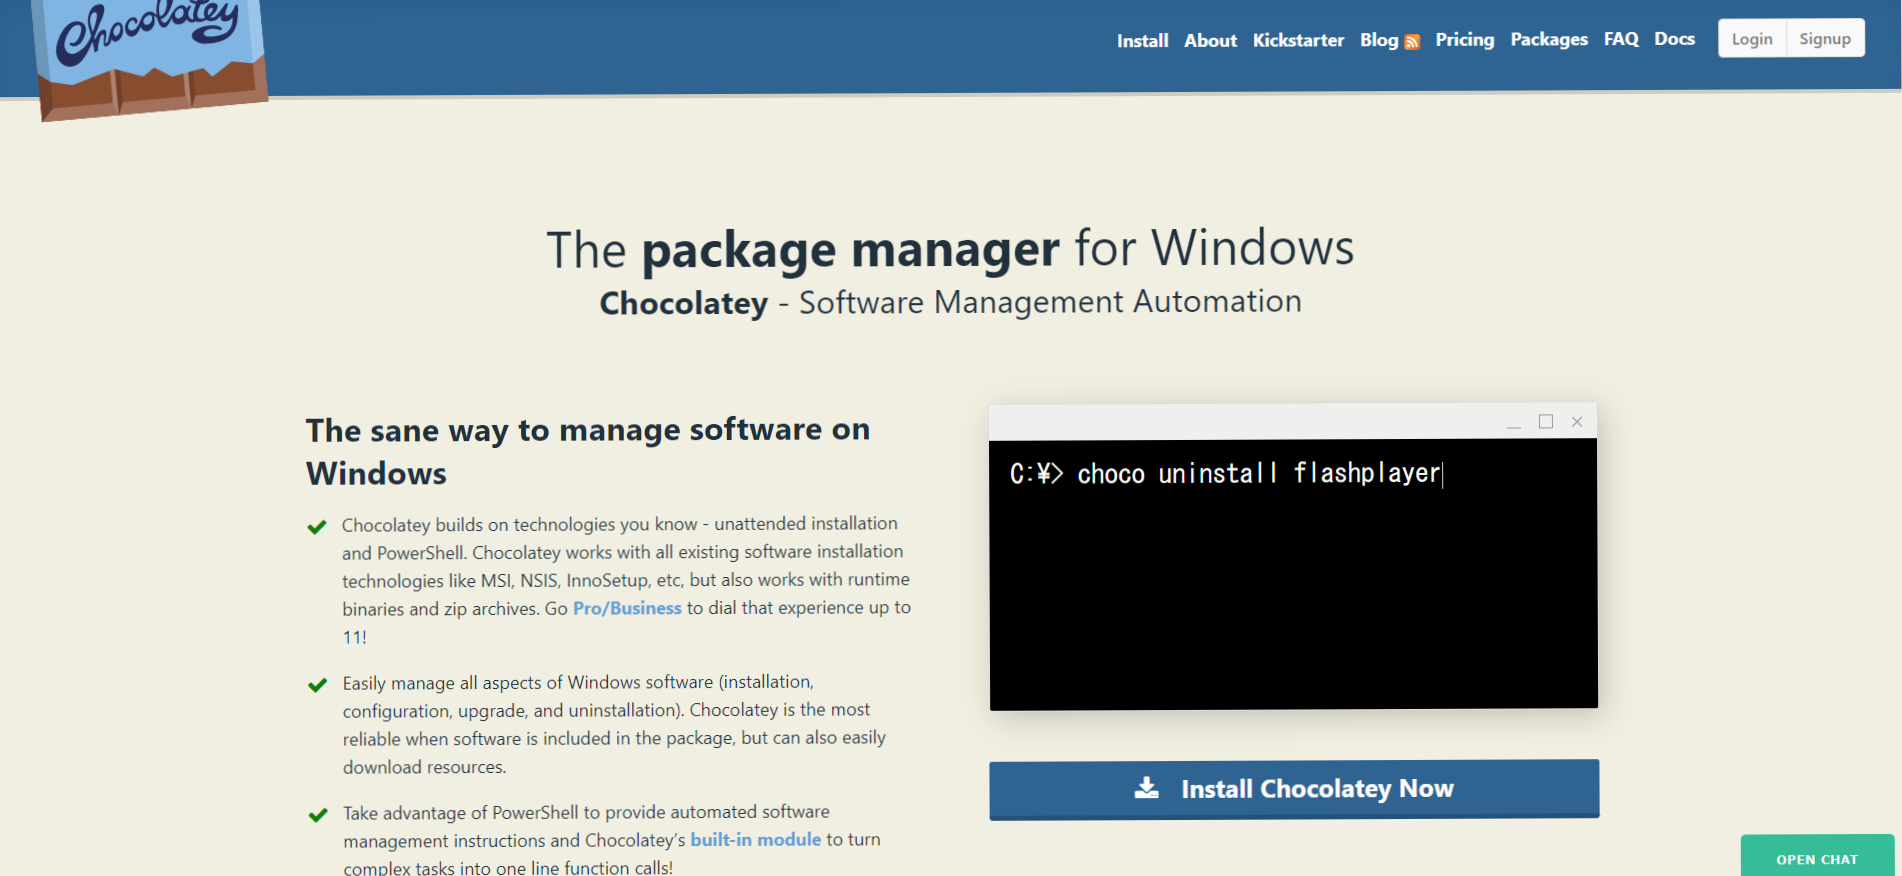
\includegraphics[width=11cm]{04.png}
\caption{chocolateyのホームページ}\label{4}
\end{figure}

\subsection{パッケージとは}
ソフトウェアにかかわるファイル一式がまとまったものをパッケージという.「ソフトウェアにかかわるファイル」には,設定ファイルやドキュメント,プログラム本体,プログラムが動くために必要なライブラリなどが含まれます.

\subsection{choco list [packageName]}
 パッケージ検索.引数がなければすべてのパッケージを表示.
\subsection{choco list -lo [packageName] }
インストール済みのパッケージ検索.引数がなければすべてのインストール済みパッケージを表示.
\subsection{cinst [packageName]}
 指定パッケージのインストール.
\subsection{cuninst [packageName]}
 指定パッケージのアンインストール.
\subsection{cup}
 Chocolatey本体のアップデート.
\subsection{cup [packageName]}
 指定パッケージのアップデート.
\subsection{cup all}
 インストール済みのパッケージを全てアップデート.
\clearpage

\section{Oracle VM VirtualBoxとは}
Oracle VM VirtualBox(以下,VirtualBoxと表記する)は,使用しているPCマシン上に仮想的なマシンを作成し,別のOSをインストール・実行することができるオープンソースソフトウェアである.WindowsやMac OS X,Linux等,様々なOSで利用することができる.
VirtualBoxをインストールしたPCのこと.
\begin{figure}[htb]
\centering

\includegraphics[width=11cm]{05.png}
\caption{VirtualBoxのイメージ}\label{5}
\end{figure}

\subsection{ホストOS}
VirtualBoxをインストールしたPCのOSのこと.本研究で使用するホストPCのOSはWindows 7/8.1である. 

\subsection{ゲストPC(仮想マシン)}
VirtualBoxで作成した仮想PC

\subsection{ゲストOS}
VirtualBoxで作成した仮想PCにインストールしたOSのこと.
\clearpage

\section{Vagrantとは}
Vagrant(ベイグラント)は,FLOSSの仮想開発環境構築ソフトウェアである.VirtualBoxをはじめとする仮想化ソフトウェアやChef(英語版)やSalt(英語版),Puppetといった構成管理ソフトウェアのラッパーとみなすこともできる.Vagrantを用いると構成情報を記述した設定ファイルを元に,仮想環境の構築から設定までを自動的に行うことができる.
\begin{figure}[htb]
\centering
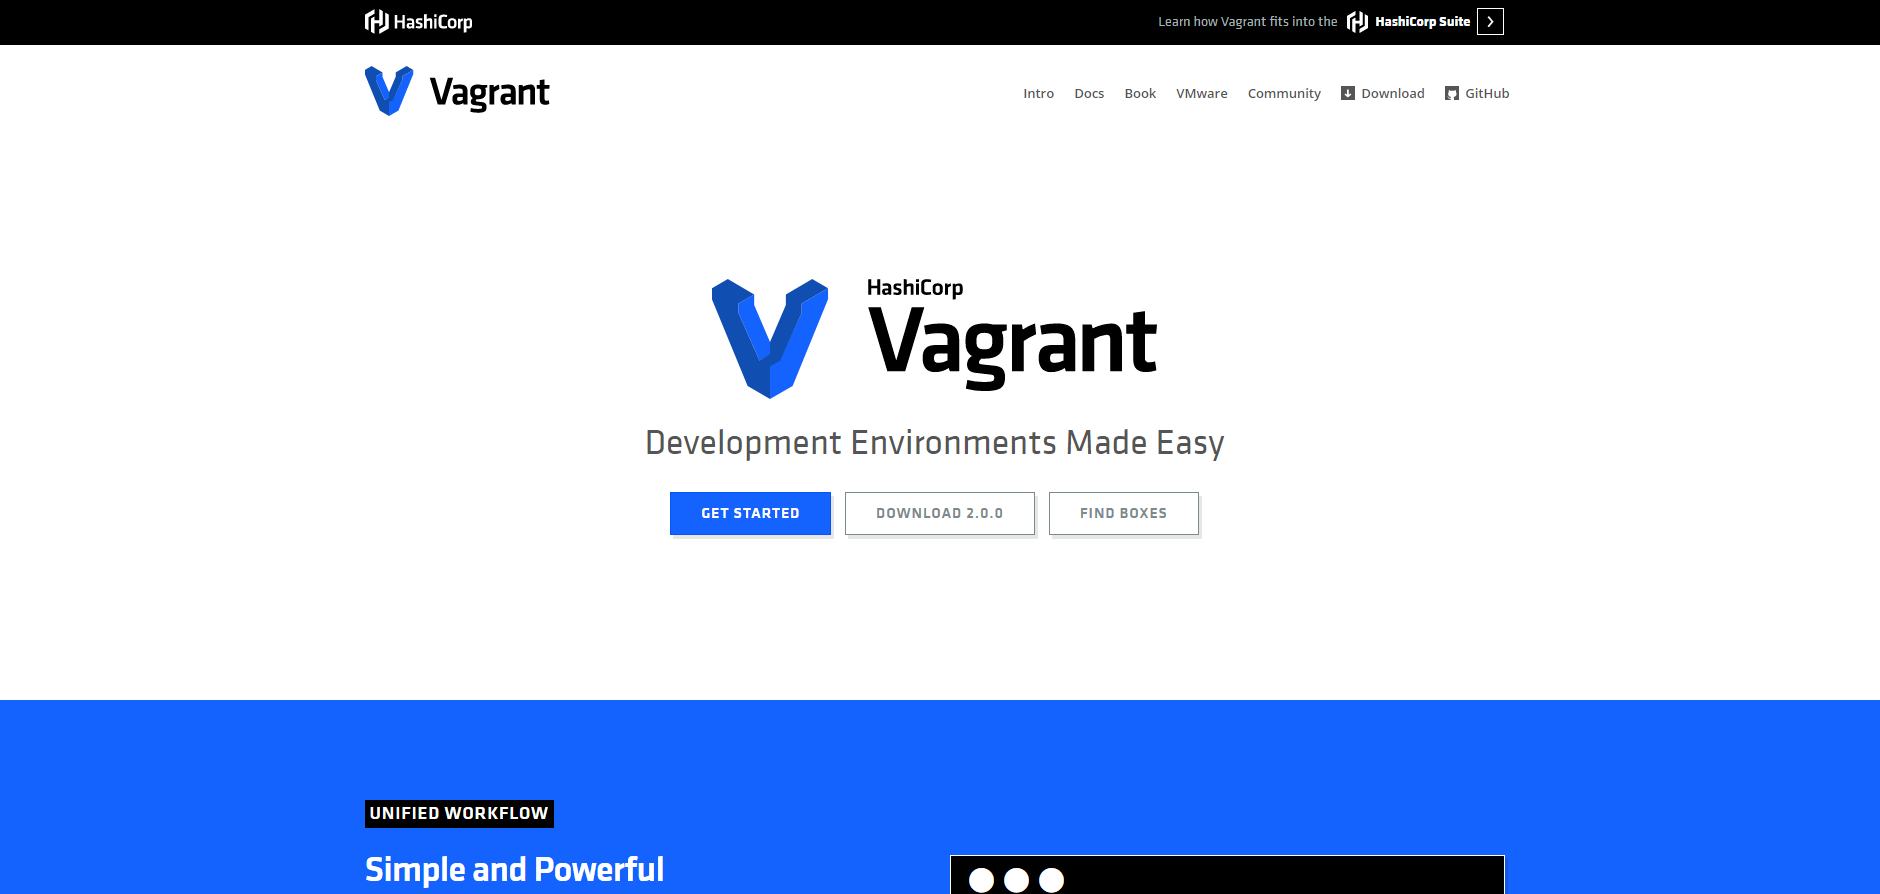
\includegraphics[width=11cm]{06.png}
\caption{Vagrantのホームページ}\label{6}
\end{figure}

\chapter{T検定について}

\section{本章の構成}
本章では本研究で使用するT検定について説明する.

\subsection{T検定とは}
帰無仮説が正しいと仮定した場合に,統計量がt分布に従うことを利用する統計学的検定法の総称である.母集団が正規分布に従うと仮定するパラメトリック検定法であり,t分布が直接もとの平均や標準偏差にはよらない(ただし自由度による)ことを利用している.2組の標本について平均に有意差があるかどうかの検定などに用いられる統計的仮説検定の一つ。日本工業規格では「検定統計量が,帰無仮説の下でt分布に従うことを仮定して行う統計的検定.」と定義している.スチューデントのt検定(Student's t-test)とも呼ばれるが,これは統計学者のウィリアム・ゴセットが雇用者であるギネスビール社に本名使用を許されずStudent というペンネームで最初の論文を発表した(1908年)ためである.


\subsection{T検定の種類}
T検定は大きく次のように分けられる.

\begin{enumerate}
\item 2つの母集団がいずれも正規分布に従うと仮定したうえでの,平均が等しいかどうかの検定.
\item 標本が対になっている,つまり1組の標本のメンバー各々ともう1組の特定のメンバーとの間に特別な関係がある場合(例えば,同じ人に前後2回調査する場合夫と妻とで比較する場合など)
\item 標本が独立で,比較する2つの群の分散が等しいと仮定できる場合(等分散性の仮定)
\item 標本が独立で,等分散性が仮定できない(異分散)場合.これは正確にはウェルチのt検定と呼ばれる.
\item 正規分布に従う母集団の平均が特定の値に等しいかどうかの検定.
\item 回帰直線の勾配が0と有意に異なるかどうかの検定.
\end{enumerate}
\newpage

\chapter{手法}

\section{全体の流れ}

本章では研究の流れについて説明する.

\begin{enumerate}
\item 開発環境の導入
\item 調査するデマツイートの決定.
\item TwitterAPIを利用できるようにOAuth認証を行う.
\item TwitterAPIを用いて日本人ユーザー50人をランダムサンプリングする.
\item TwitterAPIを用いてデマツイートをリツイートしたユーザー50人を取得する.
\item TwitterAPIを用いて集めた各ユーザーの最新100ツイートに含まれるリツイートの数を調べて,平均を計算する.
\item 日本人ユーザー50人とデマツイートをリツイートしたユーザー50人の最新100ツイートに含まれるリツイートの数の平均の差が,偶然的な誤差の範囲にあるものかどうかを判断する為に2標本T検定を行う.
\end{enumerate}

\section{開発環境の導入}

本研究では様々なソフトウェアを使用する.そのため,ソフトウェアの導入方法を解説する.

\subsection{Chocolateyの導入}
パッケージ管理システム「Chocolatey」をインストールするためには、管理者権限でコマンドプロンプトを起動する必要がある.Windows 10の場合,「スタート」ボタンを右クリックして,「コマンドプロンプト(管理者)」をクリックする.Chocolatey」をインストールするために,管理者権限で起動したコマンドプロンプトで以下のコマンドを実行する.\begin{verbatim}
@"%SystemRoot%\System32\WindowsPowerShell\v1.0\powershell.exe" -NoProfile 
-InputFormat None -ExecutionPolicy Bypass -Command "iex ((New-Object System.
Net.WebClient).DownloadString('https://chocolatey.org/install.ps1'))" && SET "
PATH=%PATH%;%ALLUSERSPROFILE%\chocolatey\bin"
\end{verbatim}

インストール完了後コマンドプロンプトを再起動して,
\texttt{clist}
と入力し,ソフトウェア一覧が表示されればインストール成功である.(時間がかかるため,\texttt{Ctrl+c}でコマンドを停止する.)インストール方法は,今後変更される可能性がある.そのため,以下のコマンドが正常に動作しない場合は,Chocolatey Galleryから最新の情報を確認してください.
\newpage

\subsection{パッケージのインストール}
「VirtualBox」と「vagrant」をChocolateyを使って,コマンドプロンプトからインストールする.「VirtualBox」と「vagrant」をインストールするために,コマンドプロンプトで,以下のコマンドを実行する.
\begin{verbatim}
$ cinst -y vagrant virtualbox
\end{verbatim}
\newpage

\subsection{Vagrantの導入}
Vagrantを使うには,Boxと呼ばれるファイルが必要になる.今回は矢吹研究室の公式マシンを使用する.

矢吹研究室公式マシンは以下のURLのGitHubリポジトリで公開されており,このリポジトリをcloneして使用する.なお,矢吹研究室公式マシンはLinuxディストリビュージョンの一つであるUbuntuを使用している.矢吹研究室公式マシンは初回起動時に様々なアプリケーションを自動でインストールする.そのため,本論文に書かれているコードを公式マシン以外で実行してもうまく動作しない可能性がある.その際は必要なアプリケーションを\texttt{apt-get install [パッケージ名]}(ubuntuの場合)でインストールすることができる.

https://github.com/yabukilab/machine

本研究では\texttt{c:/vagrant}というディレクトリにcloneする.

そうすると,\texttt{c:/vagrant/machine}下に\texttt{Vagrantfile}というファイルが存在するはずである.
存在を確認したらコマンドプロンプトで以下のコマンドを入力する.

\begin{verbatim}

cd c:\vagrant\machine

vagrant up

vagrant ssh

\end{verbatim}

これで,コマンドプロンプト上で仮想マシンにssh接続できれば成功である.
\newpage

\subsection{TwitterAPIの導入}
TwitterAPIを利用するためにはTwitterのアカウントが必要である.その為,Twitterアカウントの作成方法を説明する.
\begin{enumerate}
\item Twitterの公式ホームぺージをgoogleで検索し,Twitterのホームページに入る.
\item 図\ref{1}の画面右上にある「アカウント作成」をクリックする.
\item Twitterを使う際に必要な「ニックネーム」,「電話番号もしくはメールアドレス」,「パスワード」を記載する.その後「アカウント作成」ボタンをクリックする.
\begin{figure}[htb]
\centering
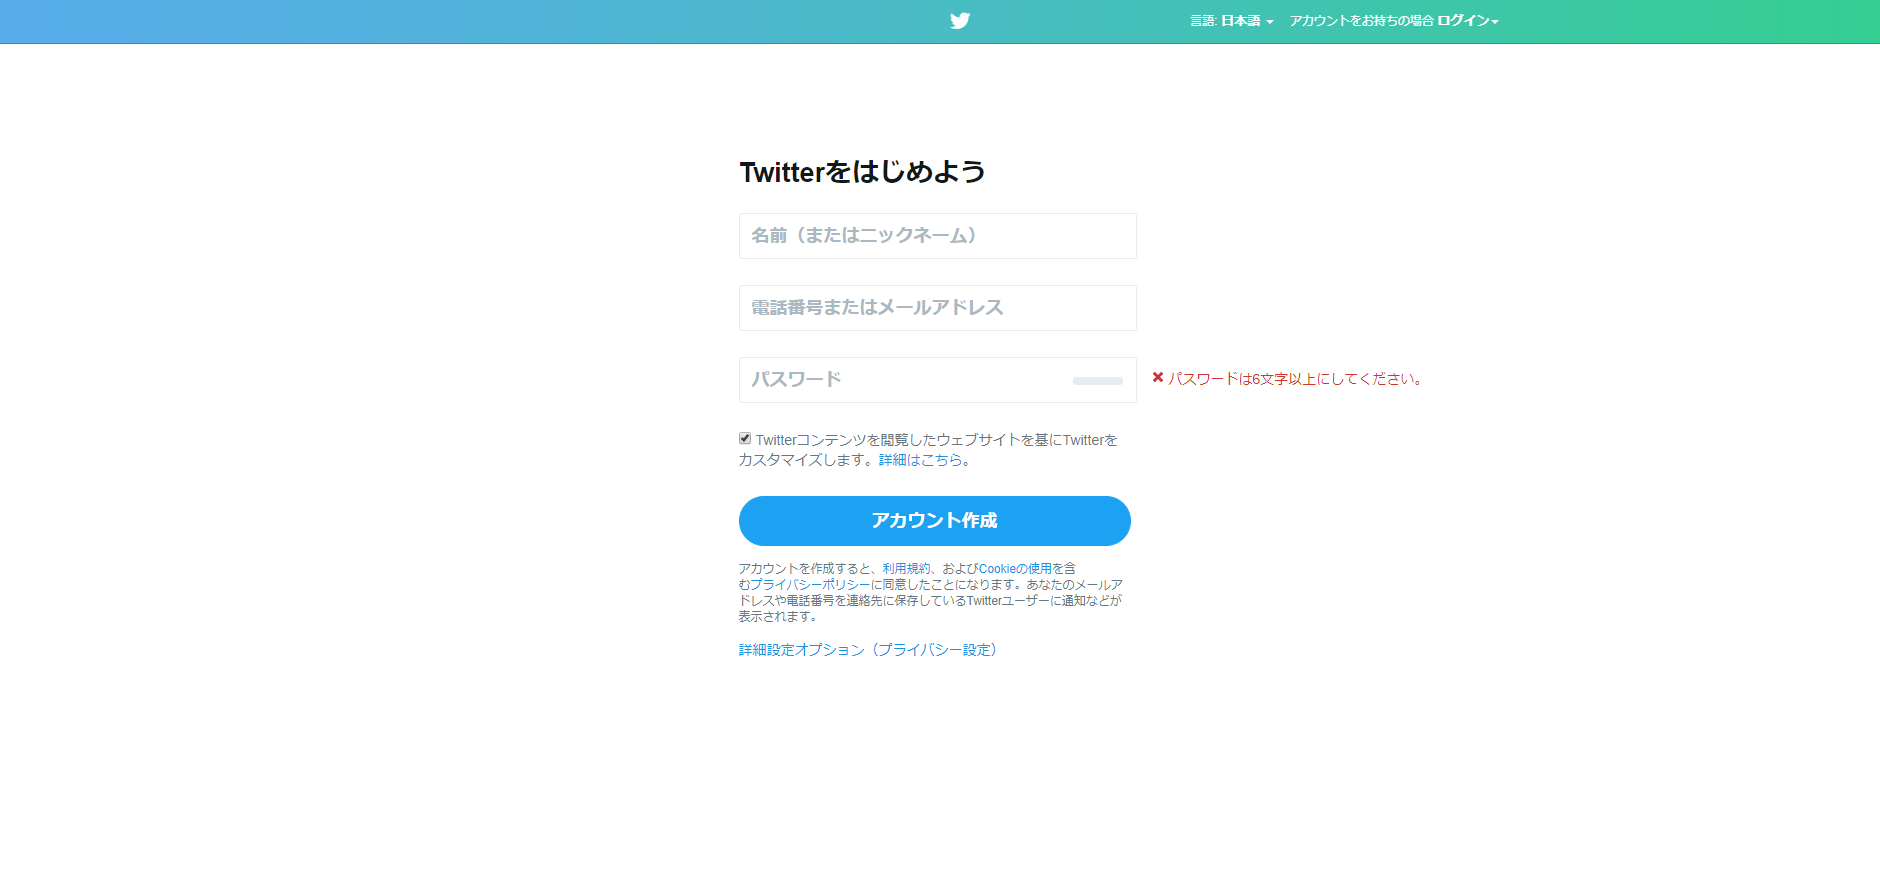
\includegraphics[width=10cm]{07.png}
\caption{アカウント作成画面}\label{7}
\end{figure}
\item ここでは電話番号の入力を要求されるが,しなくてもアカウントの登録は可能である.電話番号を入力するのであれば,電話番号の記載を.電話番号を入力しないのであれば「次へ」ボタンの左下にある「スキップ」をクリックする.
\begin{figure}[htb]
\centering
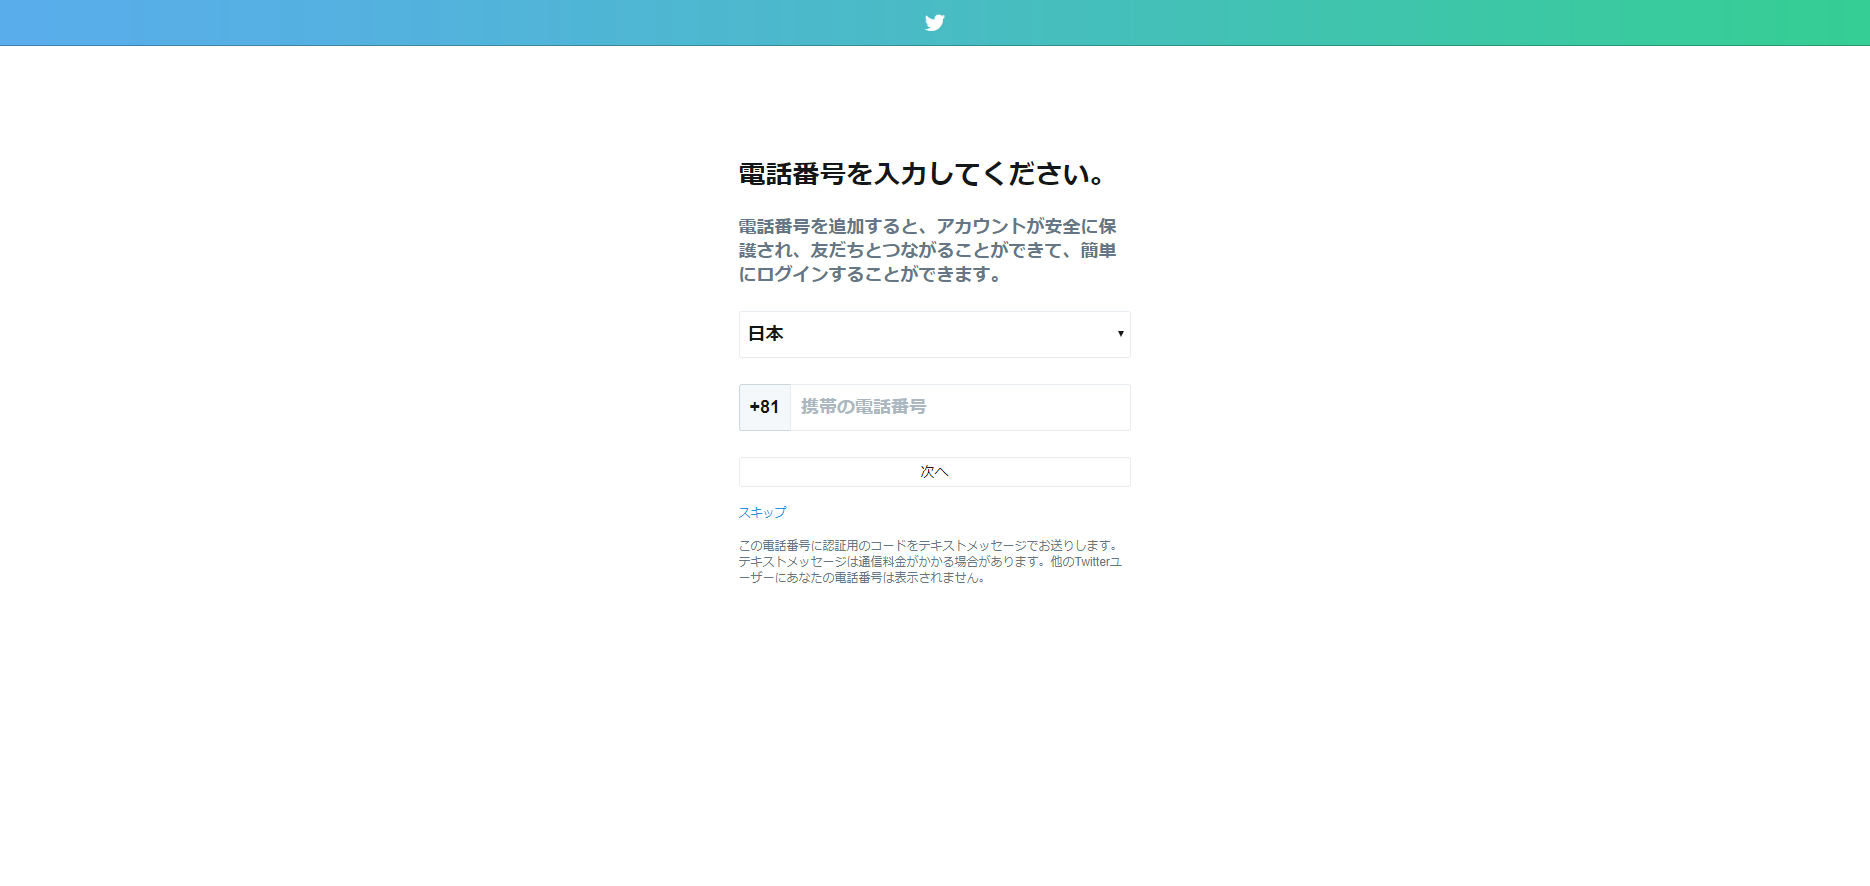
\includegraphics[width=10cm]{08.png}
\caption{電話番号入力画面}\label{8}
\end{figure}
\newpage
\item ユーザー名を記入する.もしくは利用可能なアカウント名をクリックして選ぶ.ユーザー名は登録後に変更が可能なため,その時の好きなユーザー名を記入することが出来る.また記入を行った際に,他のユーザーに使われていると記入ボックスの右隣りに「このユーザー名は既に使用されています。」と表示される.ユーザー名を決めることができたら,アカウント作成は終了である.
\begin{figure}[htb]
\centering
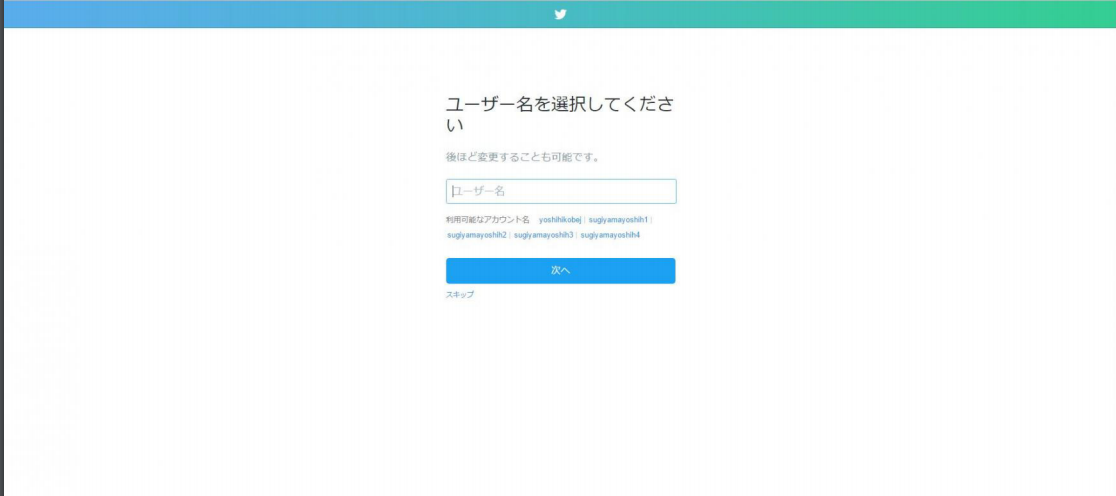
\includegraphics[width=10cm]{09.png}
\caption{ユーザー名入力画面}\label{9}
\end{figure}
\end{enumerate}

\subsubsection{Twitter API Keyの取得方法}
アプリケーションを作る際に必要になるのが,Consumer Key,Consumer Secret,Access Token,Access Token Secretの4つです.この4つを取得する方法について説明する.
\begin{enumerate}
\item https://apps.twitter.com/ にアクセスする
\item なにもアプリを作っていないと下記のような画面が出るので,Create New App ボタンをしてアプリケーションを作ります.
\begin{figure}[htb]
\centering
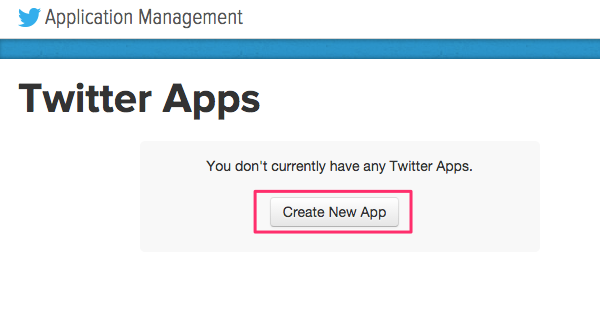
\includegraphics[width=10cm]{10.png}
\caption{アプリ作成画面1}\label{10}
\end{figure}
\item Create New App ボタンを押すと,下記のような画面が出てきます.
\begin{figure}[htb]
\centering
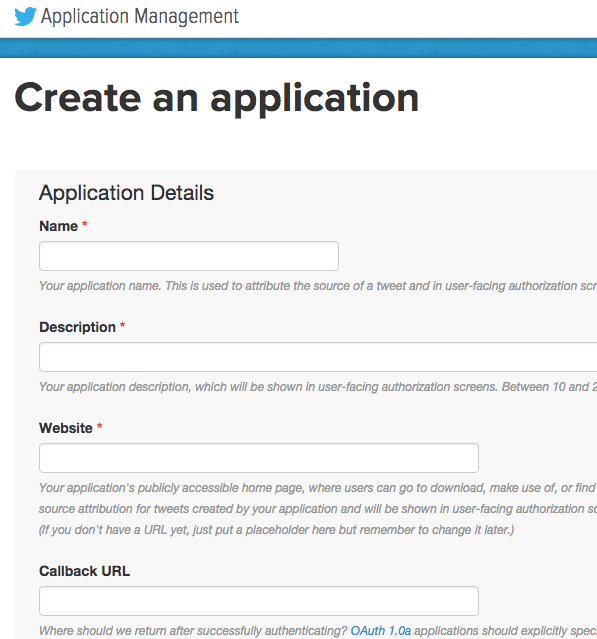
\includegraphics[width=10cm]{11.png}
\caption{アプリ作成画面2}\label{11}
\end{figure}
\item Nameにはアプリケーションの名前を入力します.文字数は32文字以内である.
\item Descriptionにはアプリケーションの説明を入力します.認証系のアプリで使う場合は認証画面にこの文言が表示されます.文字数は10文字以上200文字以下である.
\item WebsiteにはアプリケーションのURLを入力します.まだ無い場合は仮のURLでも問題ありません.
\item CallbackURLは任意の入力項目です.コールバックURL認証後に戻ってくるURLです.
\item アプリケーション作成後,アプリケーション管理画面のKeys and Access Tokensタブをクリックします.下記のような画面が表示されます.ここでConsumer KeyとConsumer Secretを取得できます.
\begin{figure}[htb]
\centering
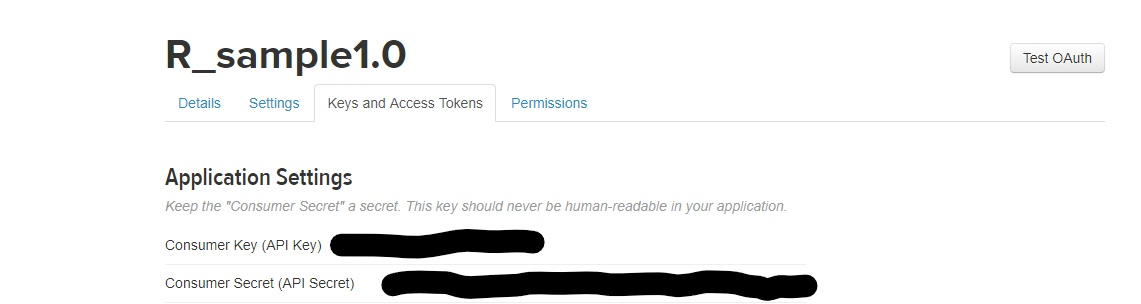
\includegraphics[width=10cm]{12.png}
\caption{Key and Access Tokens}\label{12}
\end{figure}
\newpage
\item Keys and Access Tokens画面の下部にあるCreate my access tokenボタンをクリックすると下記のような画面が表示されます.ここで, Access TokenとAccess Token Secretを取得できます.
\begin{figure}[htb]
\centering
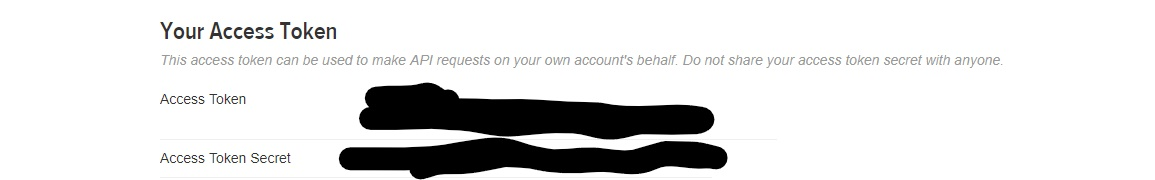
\includegraphics[width=10cm]{13.png}
\caption{Key and Access Tokens2}\label{13}
\end{figure}
\end{enumerate}

\section{調査するデマツイートの決定}
デマと断定できるツイートを調べる.今回の研究では以下の4つのデマツイートを対象に調査を行う.

\begin{figure}[htb]
\centering
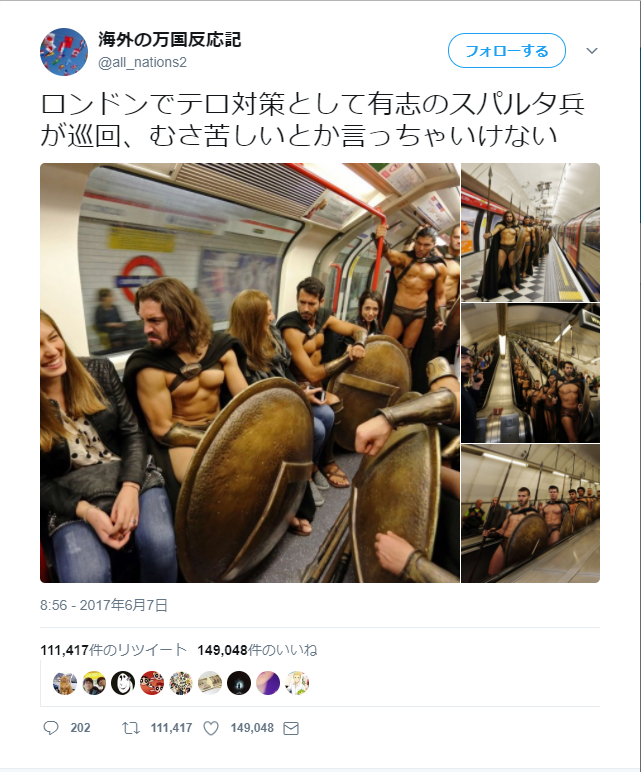
\includegraphics[width=10cm]{dema1.png}
\caption{デマツイート1}\label{14}
\end{figure}
\clearpage

\begin{figure}[htb]
\centering
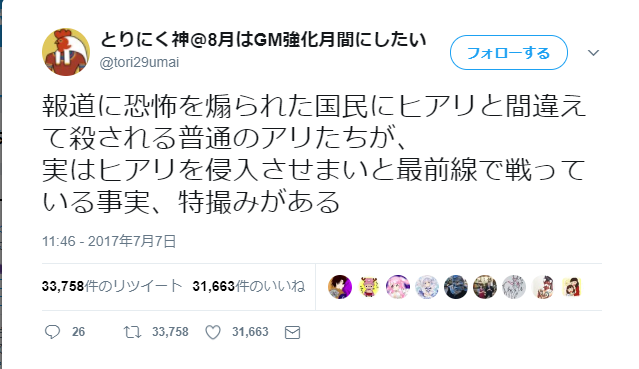
\includegraphics[width=10cm]{dema2.png}
\caption{デマツイート2}\label{15}
\end{figure}
\clearpage

\begin{figure}[htb]
\centering
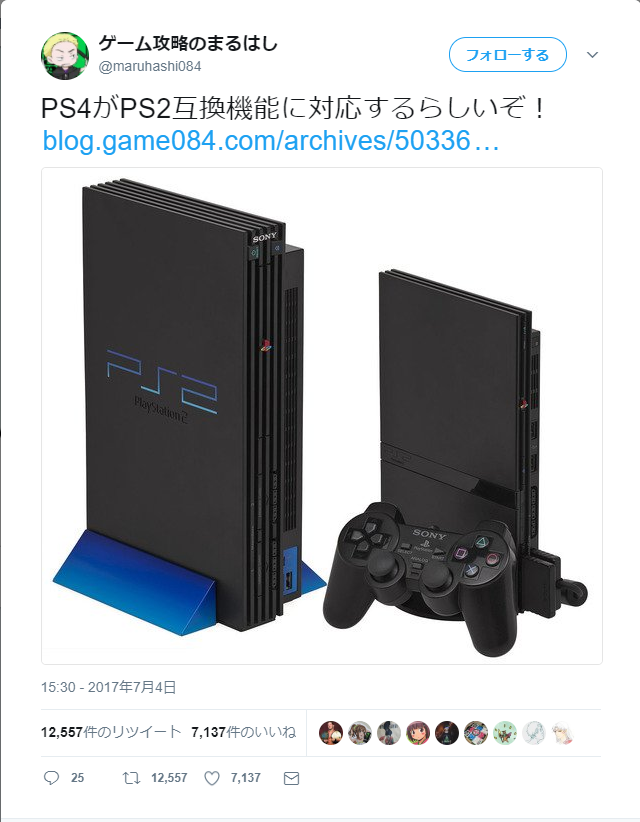
\includegraphics[width=10cm]{dema3.png}
\caption{デマツイート3}\label{16}
\end{figure}
\clearpage

\begin{figure}[htb]
\centering
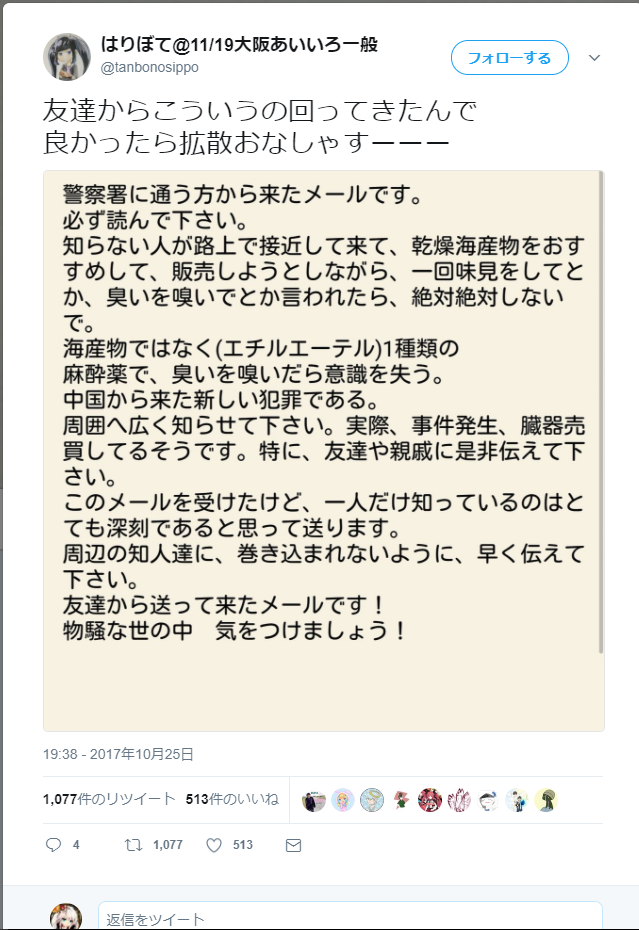
\includegraphics[width=10cm]{dema4.png}
\caption{デマツイート4}\label{17}
\end{figure}

以上の4つのデマツイートの詳細を以下に示す.
\begin{itemize}
 \item デマツイート1として,ロンドンのテロ対策で有志のスパルタ兵が巡回しているというデマツイートがある.実際は映画の宣伝である.(TweetID:872255950131822596)
 \item デマツイート2として,国内のアリがヒアリに対抗出来るというデマツイートがある.実際は誤情報である.(TweetID:883170290242527232)
 \item デマツイート3として,PS4にPS2互換機能対応するというデマツイートがある.実際は誤情報である.(TweetID:882139486968205312)
 \item デマツイート4として,路上で乾燥海産物を売る人がいるが,それは麻酔薬で匂いを嗅いだら意識を失うというデマツイートがある.実際は昔韓国で流行したデマの内容と同じものである.(TweetID:923151745923948545)
\end{itemize}



\section{Oauth認証のやり方}
\begin{enumerate}
\item 以下のコードを入力する.ファイル名はauth.pyとする.
\begin{verbatim}
# -*- coding: utf-8 -*-

import tweepy

consumer_key = ""#引用符の中にconsumer_keyの情報を記述する
consumer_secret = ""#引用符の中にconsumer_secretの情報を記述する

access_token = ""#引用符の中にaccess_tokenの情報を記述する
access_token_secret = ""#引用符の中にaccess_token_secretの情報を記述する

auth = tweepy.OAuthHandler(consumer_key, consumer_secret)
auth.set_access_token(access_token, access_token_secret)
api = tweepy.API(auth)
\end{verbatim}
\item vagrantにssh接続した状態で
\begin{verbatim}
sudo apt-get install python-setuptools python-pip
sudo easy_install tweepy
\end{verbatim}
を入力し,インストールを行う.
\item 正常にインストールが行われたのを確認したら,vagrantにsshで接続した状態で
\begin{verbatim}
python auth.pyを実行する.
\end{verbatim}
\item 何もコマンドプロンプト上に表示されなければOauth認証成功である.
\end{enumerate}

\section{TwitterAPIを用いたデータ収集方法}

本章では研究で使用するデータを収集する方法の説明をする.

\subsection{日本人ユーザー50人をランダムサンプリングする方法}
\begin{enumerate}
\item 以下のコードを入力する.ファイル名はranjp.pyとする.
\begin{verbatim}
# -*- coding: utf-8 -*-

import twitter
import sqlite3
from random import randint

api = twitter.Api()
count = 0
while count < 50:
    i = randint(1,500000000)
    try:
        user = api.GetUser(i)
    except:
        continue
    if user.time_zone in [u'Osaka', u'Tokyo', u'Sapporo']:
        con.execute('insert into data values (%s, %s, %s)' % (user.statuses_count, user.friends_count, user.followers_count))
        count += 1
        con.commit()

con.close()
\end{verbatim}
\item vagrantにssh接続した状態で
\begin{verbatim}
python ranjp.py
\end{verbatim}
を実行する.
\item 結果が出力されれば成功である.
\end{enumerate}
\newpage

\subsection{デマツイートをリツイートしたユーザー50人を取得する方法}
\begin{enumerate}
\item 以下のコードを入力する.ファイル名はrtlist.pyとする.
\begin{verbatim}
# -*- coding: utf-8 -*-

import tweepy
import json
import sys
from pprint import pprint
from auth import api

for line in sys.stdin:
  tweetId = line.rstrip()
  sys.stderr.write("checking retweeters of %s...\n" % tweetId)

  リツイートした人を調べたことを記録する。
  sys.stdout.write("update retweets set retweetersChecked=true where id=%s;\n" % (tweetId))

  try:
    retweeters = api.retweets(tweetId,100)
    for t in retweeters:
     このオブジェクトの中身がわかりにくい。(PyDevのデバッガで調べた。)
      user = t.user
      userId = user.id_str
      screenName = user.screen_name

      sys.stdout.write("values (%s,'%s');\n" % (userId, screenName))#これは重複エラーになるはず
    sys.stdout.flush()
  except:
    pass
\end{verbatim}
\item vagrantにssh接続した状態で
\begin{verbatim}
echo tweetid(ツイート固有のIDのこと) | python rtlist.py
\end{verbatim}
を実行する.
\item 結果が出力されれば成功である.
\end{enumerate}

\section{2標本T検定の方法}
本章では,日本人ユーザー50人とデマツイートをリツイートしたユーザー50人の最新100ツイートに含まれるリツイートの数の平均の差が,偶然的な誤差の範囲にあるものかどうかを判断する為に2標本T検定を行う方法を説明する.

\subsection{データの対応の有無}
t検定は2つのグループの平均の差が偶然誤差の範囲内にあるかどうかを調べるものである.まず,データに対応があるかどうかでt検定のやり方が変わってくる.今回は全ての組み合わせでデータの対応がないため,各グループの平均と分散だけからt検定を行うことになる.分散がほぼ等しいと見なせる場合と分散が等しいとは見なせない場合に応じて,各々「分散が等しいときのt検定」「分散が等しくないときのt検定」を適用する.分散が等しいかどうかの判断はF検定によって行う.

\subsection{F検定の方法}
以下のデータは日本人ユーザー50人とデマツイート1をリツイートしたユーザー50人の最新100ツイートに含まれるリツイートの数である.このデータを使ってF検定の方法を説明する.
\begin{verbatim}
デマ1	ランダム日本人ユーザー
70	45
21	19
3	26
81	19
81	33
27	15
23	20
44	20
76	14
41	4
100	24
19	25
55	39
55	26
20	45
99	4
73	29
57	9
69	15
27	2
24	9
98	9
99	38
36	16
30	8
32	28
95	45
74	36
67	30
62	15
72	11
86	6
48	1
64	55
57	26
94	89
26	73
94	9
90	13
63	2
54	11
49	4
37	0
70	1
92	0
13	7
71	9
34	12
61	0
1	6
\end{verbatim}
\clearpage

\begin{figure}[htb]
\centering
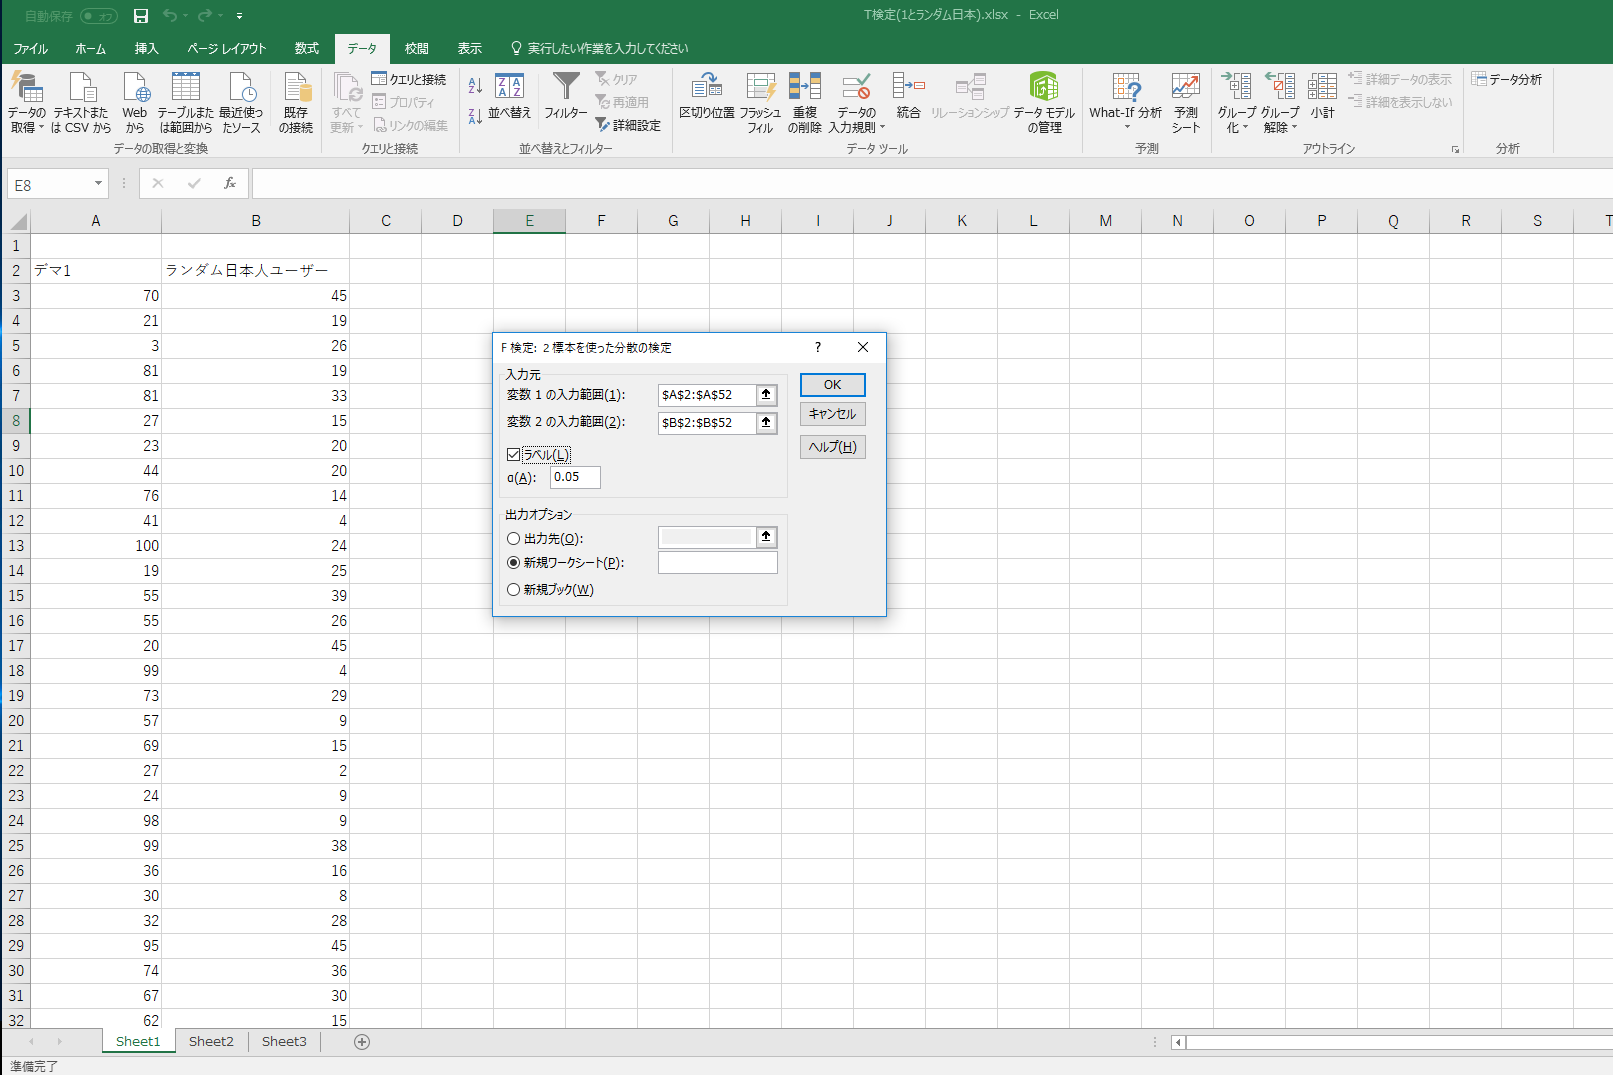
\includegraphics[width=13cm]{f1.png}
\caption{F検定}\label{18}
\end{figure}
Excelのデータタブを開きデータ分析の項目をクリックし,F検定:2標本を使った分散の検定を選択.変数1の入力範囲としてデマツイート1のデータ全て.変数2の入力範囲としてランダム日本人ユーザー全てを選択する.ラベルにチェックを入れ,aを0.05に設定する.OKをクリックすると結果が表示される.
\clearpage

\begin{figure}[htb]
\centering
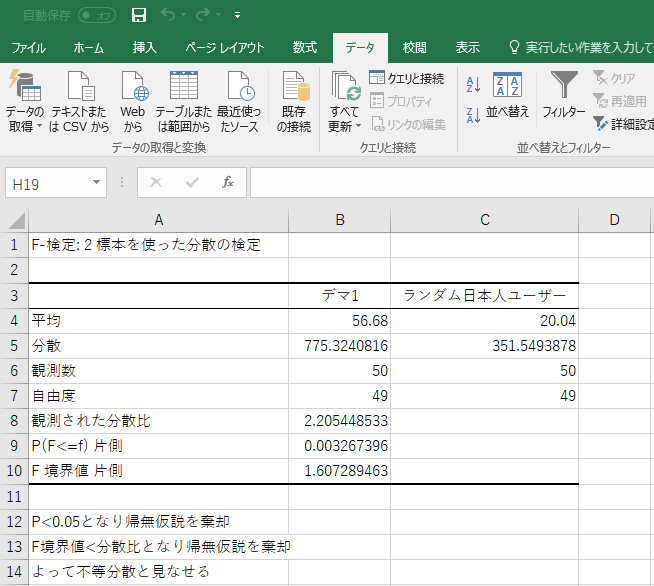
\includegraphics[width=13cm]{f2.png}
\caption{F検定結果}\label{19}
\end{figure}
結果から不等分散であることが分かった.次項にて同じデータを例に2標本t検定の方法を説明する.
\clearpage

\subsection{2標本t検定の方法}
\begin{figure}[htb]
\centering
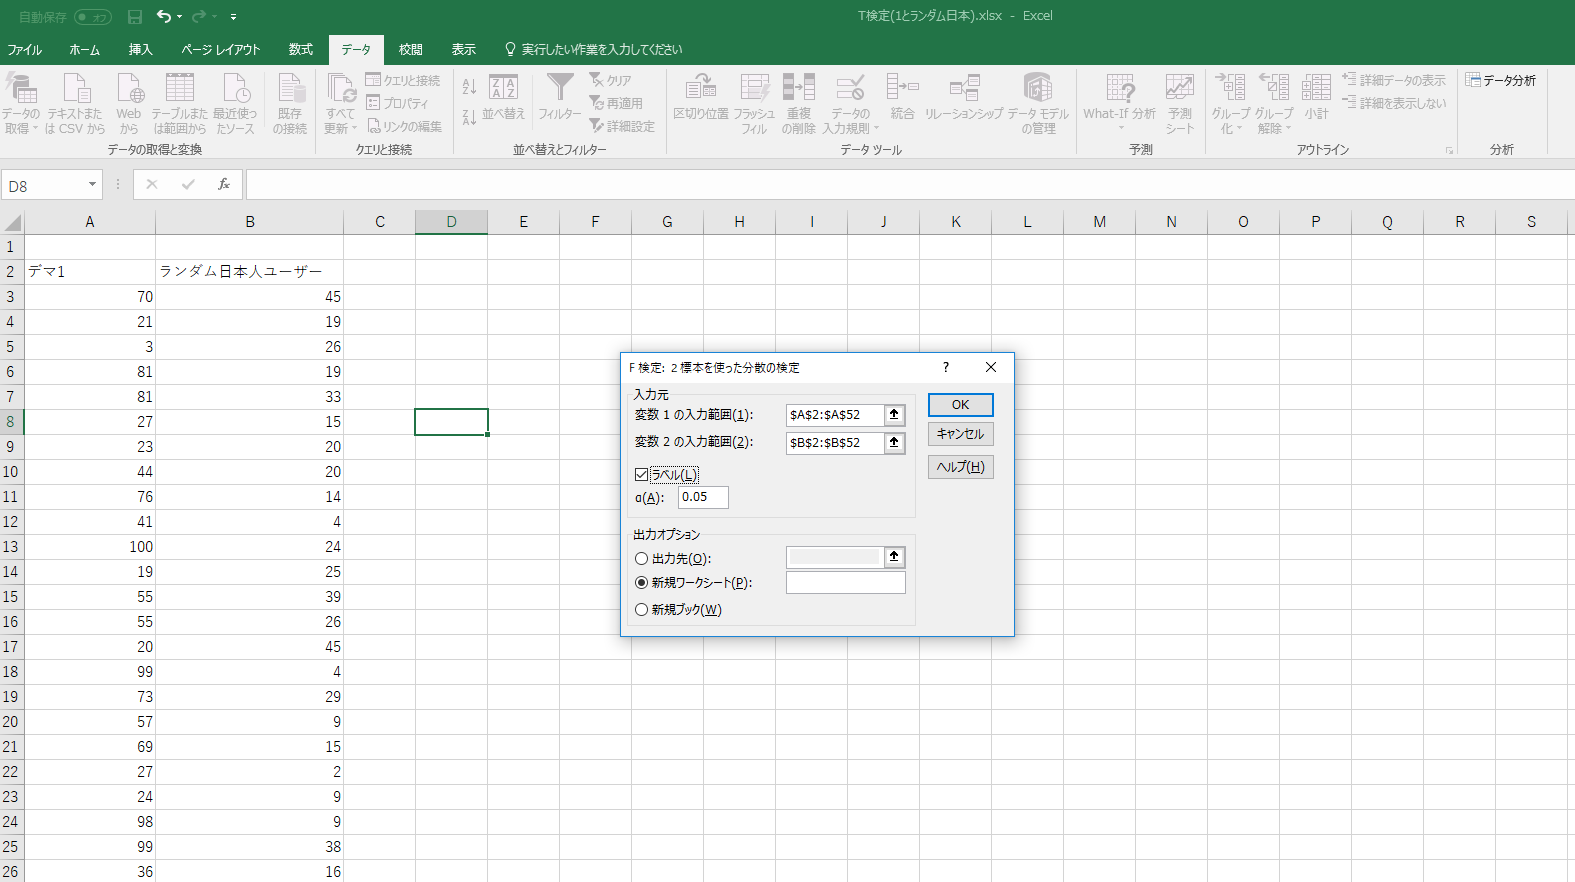
\includegraphics[width=13cm]{t1.png}
\caption{t検定}\label{20}
\end{figure}
Excelのデータタブを開きデータ分析の項目をクリックし,t検定:分散が等しくないと仮定した2標本による検定を選択.変数1の入力範囲としてデマツイート1のデータ全て.変数2の入力範囲としてランダム日本人ユーザー全てを選択する.ラベルにチェックを入れ,aを0.05に設定する.OKをクリックすると結果が表示される.
\clearpage

\begin{figure}[htb]
\centering
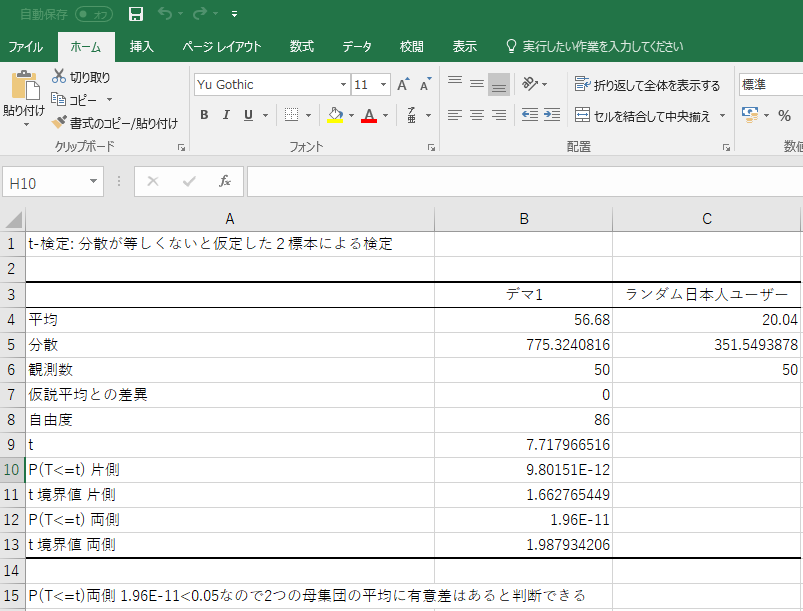
\includegraphics[width=13cm]{t2.png}
\caption{t検定結果}\label{21}
\end{figure}
結果から2つの母集団の平均に有意差はあると分かった.
\clearpage

\chapter{結果}
\section{日本人ユーザ50人をランダムサンプリングした結果}
日本人ユーザ50人をランダムサンプリングした結果以下のようになった.
\begin{verbatim}
ランダムに取得した日本人ユーザ,直近100ツイートのRT数
myaowmyaow0503	,45
karasukun_,19
Toradora_ryo,26
subakura______8,19
star_hibiki,33
minsu519,15
m_arimo0,20
ao_tyou,20
xMeq__,14
spla_balsamico,4
Kmnoka43,24
ngbba06,25
kzk_PC,39
a__xxx,26
spdk5yn9miki,45
JAfoINY3Czn4LV4,4
__zxwy,29
blacklotus_krhs,9
boncalpis,15
marchan_impulse,2
yellow____1103,9
usss___umi,9
Miu_NGZ4602,38
tora_prpr,16
yumehiko_mugen,8
HACHIGORO2011,28
kk_cain,45
chii___ms,36
fog_wolves,30
sqUmSkAnqmSjhUF,15
sd_Ikeda_Luna,11
rarirarimann,6
howusee_it70,1
mrsk_o3o,55
i__k0603,26
rikuxsakura,89
kaho05,73
ryhki,9
hagi28,13
atlach_nacha495,2
yuniba258,11
okusaredori,4
hizidsa,0
SteedVLX,1
10ac_mttk,0
mw_92184,7
ichiha1126,9
825524_rin,12
haruka_syue,0
EcNami,6
\end{verbatim}
\clearpage

\begin{figure}[htb]
\centering
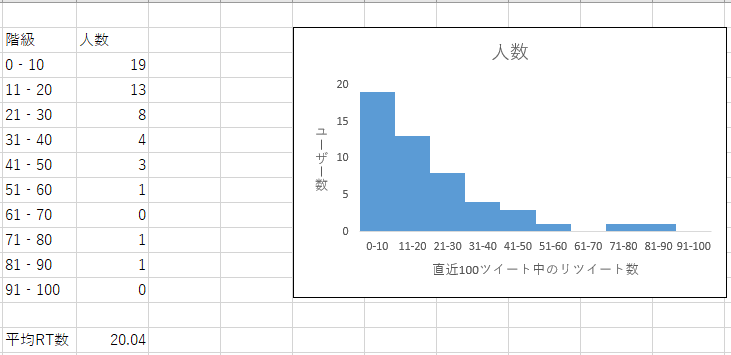
\includegraphics[clip,width=15cm,height=9cm]{ranjp.png}
\caption{日本人ユーザ50人の平均RT数とヒストグラム}\label{22}
\end{figure}
\clearpage

\section{デマツイート1をリツイートしたユーザー50人を取得した結果}
デマツイート1をリツイートしたユーザー50人を取得した結果以下のようになった.
\begin{verbatim}
デマツイート1をRTしたユーザー,直近100ツイートのRT数
mnmnssk,70
yu612keisei86,21
poohshan7427,3
Yuion0016871,81
EX24TA,81
ohta_isan_,27
rassyrassy333,23
BlueMAX_VJ,44
piyo2jack,76
atuto__,41
izumo_abc,100
Anmr118,19
teruteruterutti,55
QqQbc,55
Akaiyu_yuki,20
sayo_candy,99
generalfrost_6,73
aiki_kc,57
masayuki311,69
shisyotosyo,27
yasui0324,24
8_wtkq,98
anewstart559,99
kazuki_hami,36
yeahtwmjgw,30
saigyoa,32
mutu_matu01,95
nmemaksumlk,74
saka_s1127,67
ossan_dai,62
yuta22074,72
jihh00,86
DnrodReds,48
yukinyoooooooon,64
ncruncham,57
qeg5P03kABpgx9X,94
muginami_nolito,26
toshi2497315,94
masash1324xx88,90
bivibeau,63
ntake1966,54
akiya_kiu,49
mamo_wa0608,37
kokonoeringo05,70
Fluorumium,92
naukosi,13
okashi_tabenai,71
gu_tara12yume,34
KotobukiSonbe,61
sudachi_1993,1
\end{verbatim}
\clearpage

\begin{figure}[htb]
\centering
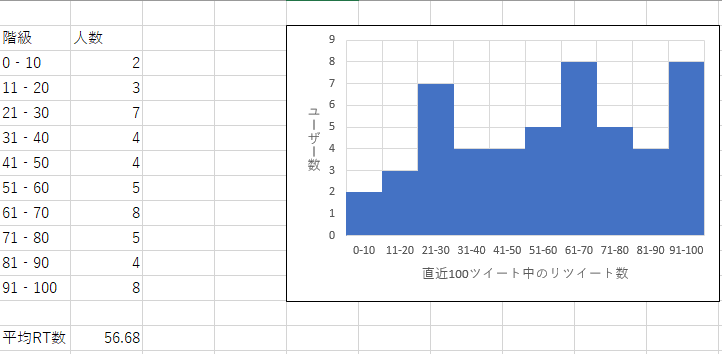
\includegraphics[clip,width=15cm,height=9cm]{d1.png}
\caption{デマツイート1をリツイートしたユーザー50人の平均RT数とヒストグラム}\label{23}
\end{figure}
\clearpage

\section{デマツイート2をリツイートしたユーザー50人を取得した結果}
デマツイート2をリツイートしたユーザー50人を取得した結果以下のようになった.
\begin{verbatim}
デマツイート2をRTしたユーザー,直近100ツイートのRT数
mmm_sheep,25
karan_1126,58
peachmint753,85
choc8o_o8,52
1010__,17
koutyou_03,95
Aliiiis_,36
nishinosonoyo,58
Ares_Vermillion,94
motipeen_424,60
sihugonomi,98
nazuna17,88
rasetunkamen,85
kotatubutonn018,76
B_M_Graphix,100
floral00,78
MkGftf,100
namako1221yu,14
moto_oolong_tea,83
cnnwp051,89
oita_shukuri,82
recureat,32
mocha_ras,100
zmdmrg,100
RYUGASAKI_Akira,28
goumonnkigu,88
NPO94867351,13
tatew3druk3,30
SSSSPIRALLIFE,76
asuka_toritori,85
AnatH_69,31
applegesu12,43
bettyboo_redeye,48
o_mocco,2
dazjelly,23
curacco,20
kabech,11
tibikkohime,18
aohina_1023,94
KoizumiRiver,86
isana777,67
ahirumaru88,98
kairidei,58
heta0alisa,64
zitomemania,93
DerBlauer_Vogel,89
26Gbs,75
harumi21kugyu11,66
saigusaalter11,49
misatsuki,72
\end{verbatim}
\clearpage

\begin{figure}[htb]
\centering
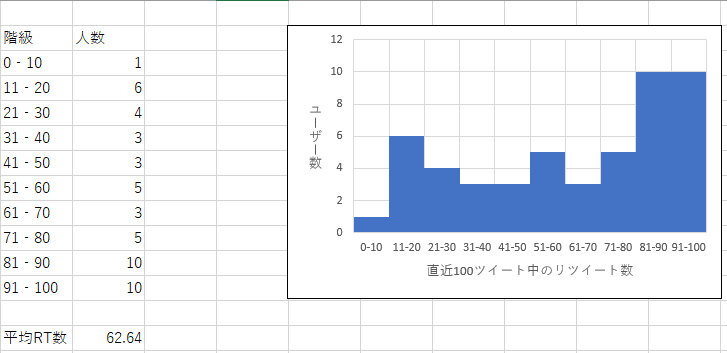
\includegraphics[clip,width=15cm,height=9cm]{d2.png}
\caption{デマツイート2をリツイートしたユーザー50人の平均RT数とヒストグラム}\label{24}
\end{figure}
\clearpage

\section{デマツイート3をリツイートしたユーザー50人を取得した結果}
デマツイート3をリツイートしたユーザー50人を取得した結果以下のようになった.
\begin{verbatim}
デマツイート3をRTしたユーザー,直近100ツイートのRT数
amaminoya,39
province_mrba,54
DoLcs888,98
Bea5851,54
tetugunn,92
rFTgM63P18EJ2BA,41
bisuko_12,28
kaneko_chang,28
fuu_mst,48
cmtaka124,99
VittoBennetPso2,91
onkyo22yoshiki,48
ChihironYY,8
kitauming,65
iria1013yd,90
shiki3861,80
BWorld1016,48
wing34nina,67
raiji3510,57
yama_oki_,84
itkr__,54
lllPembrokelll,3
seojin_ksjim35,100
chiico33,45
_HHH__,56
rizain1192,93
groovenUG,98
iiwashi69pantu,27
n_woE,53
tuji_gami,52
nui_896,36
mijimiji05,12
Kookie_Jams,94
hana2657,100
nakayama_GOGO,48
kgmnkzklrn,74
12Rrg,67
zoiqq009,47
Bboycaramel0413,50
paxcco,29
tarezousan47,55
purebreed1,78
vervkwsm,79
kk_segreto,34
magamirei7,25
oogamikotarou,26
Jyeido_Rezary,81
SIKI_495,90
yama_824,41
sola_sk_0,57
\end{verbatim}
\clearpage

\begin{figure}[htb]
\centering
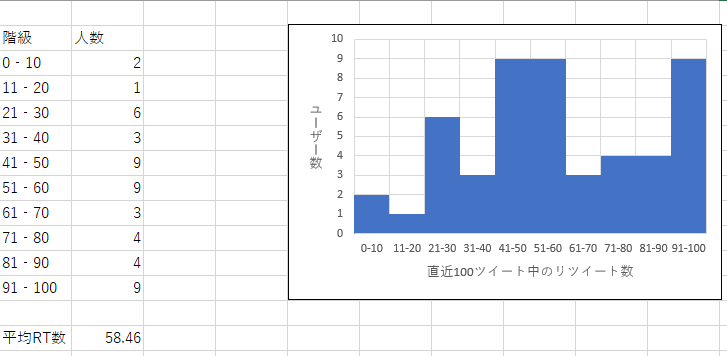
\includegraphics[clip,width=15cm,height=9cm]{d3.png}
\caption{デマツイート3をリツイートしたユーザー50人の平均RT数とヒストグラム}\label{25}
\end{figure}
\clearpage

\section{デマツイート4をリツイートしたユーザー50人を取得した結果}
デマツイート4をリツイートしたユーザー50人を取得した結果以下のようになった.
\begin{verbatim}
デマツイート4をRTしたユーザー,直近100ツイートのRT数
noncats,72
ruusan203,43
Choco_tGZep3q,21
WolfHound_M40A3,87
suchas1219n,87
yzmkn_2804,60
wahuxu_1002,48
fisss_,10
mimohako_0616,15
wallcroft039400,10
OpBnT9Sdre7jCUJ,49
kai_akatuki,91
mina0701kana11,30
UK_Arther,44
6moonH,86
rihama_tukumo99,13
pet_shimobe,44
f9u6yq,82
krmr613,21
zakokyara1112,48
otz_69,37
rin0613neya,20
6loSYqgdfJmFQjP,100
htH61uAJexXFloZ,98
chipakan,93
totoko1981,93
ozigisou1028,94
sonicstar3739,74
zounitoburi,26
k66yukina,36
crimsondolls,66
1010yazukide41,96
ZjMsy,95
kituneme_,72
rena__rena__re,61
ventwo_two,60
kisaragisuzuma7,59
kin_102,65
kuisinboo24,54
0yHUkIgVjjbwOU4,90
Iliyaerja,49
younnri,49
dddaaa315,72
mizubonarigatou,46
GilgitGlaucous,89
sakurablue1126,78
early_ana_,95
fakeshe,30
FC_Nekomaturi,25
AlithinCOF,13
\end{verbatim}
\clearpage

\begin{figure}[htb]
\centering
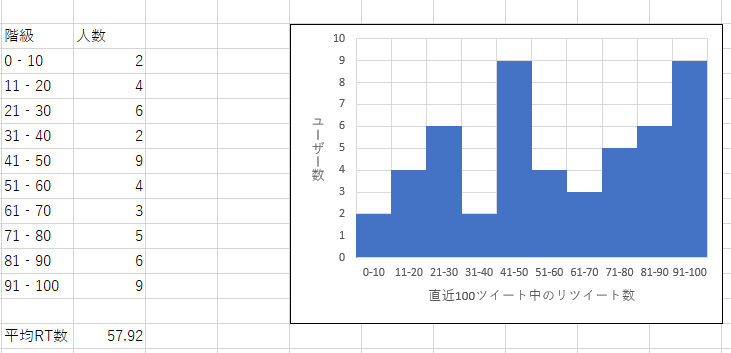
\includegraphics[clip,width=15cm,height=9cm]{d4.png}
\caption{デマツイート4をリツイートしたユーザー50人の平均RT数とヒストグラム}\label{26}
\end{figure}
\clearpage

\section{F検定の結果1}
ランダムサンプリングした日本人ユーザー50人とデマツイート1をリツイートしたユーザー50人の最新100ツイートに含まれるリツイートの数でF検定を行った結果を以下に示す.

\begin{figure}[htb]
\centering
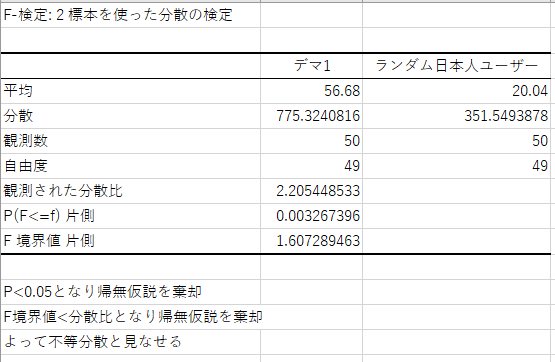
\includegraphics[width=13cm]{14.png}
\caption{F検定結果1}\label{27}
\end{figure}
\clearpage

\section{F検定の結果2}
ランダムサンプリングした日本人ユーザー50人とデマツイート2をリツイートしたユーザー50人の最新100ツイートに含まれるリツイートの数でF検定を行った結果を以下に示す.

\begin{figure}[htb]
\centering
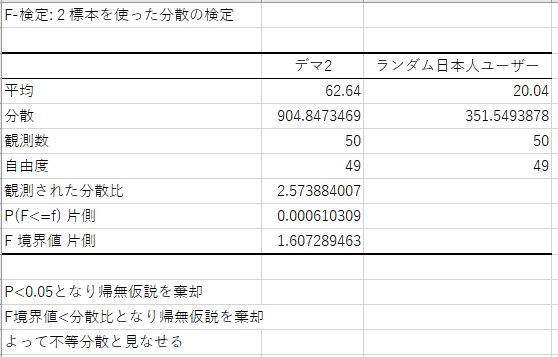
\includegraphics[width=13cm]{15.png}
\caption{F検定結果2}\label{28}
\end{figure}
\clearpage

\section{F検定の結果3}
ランダムサンプリングした日本人ユーザー50人とデマツイート3をリツイートしたユーザー50人の最新100ツイートに含まれるリツイートの数でF検定を行った結果を以下に示す.

\begin{figure}[htb]
\centering
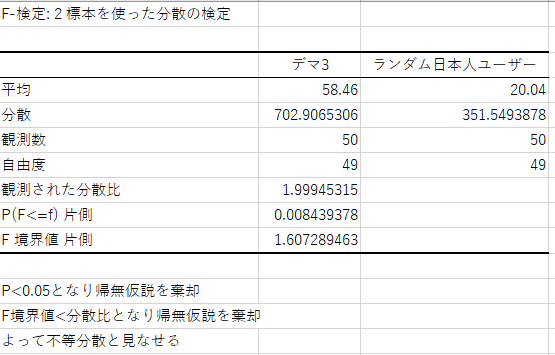
\includegraphics[width=13cm]{16.png}
\caption{F検定結果3}\label{28}
\end{figure}
\clearpage

\section{F検定の結果4}
ランダムサンプリングした日本人ユーザー50人とデマツイート4をリツイートしたユーザー50人の最新100ツイートに含まれるリツイートの数でF検定を行った結果を以下に示す.

\begin{figure}[htb]
\centering
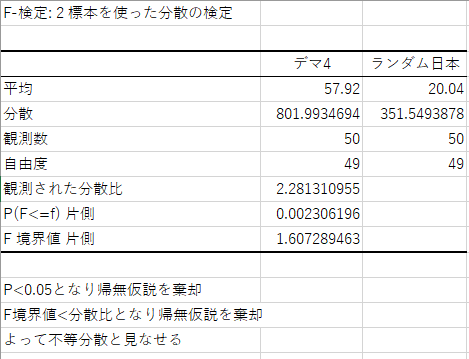
\includegraphics[width=13cm]{17.png}
\caption{F検定結果4}\label{29}
\end{figure}
\clearpage

\section{2標本t検定の結果1}
ランダムサンプリングした日本人ユーザー50人とデマツイート1をリツイートしたユーザー50人の最新100ツイートに含まれるリツイートの数で2標本t検定を行った結果を以下に示す.

\begin{figure}[htb]
\centering
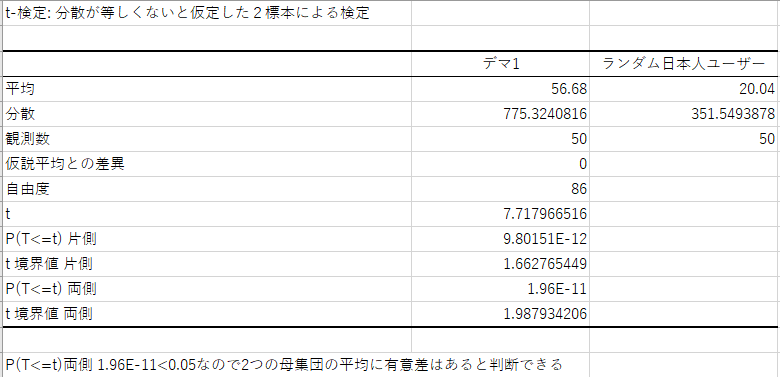
\includegraphics[width=13cm]{18.png}
\caption{t検定結果1}\label{30}
\end{figure}
\clearpage

\section{2標本t検定の結果2}
ランダムサンプリングした日本人ユーザー50人とデマツイート2をリツイートしたユーザー50人の最新100ツイートに含まれるリツイートの数で2標本t検定を行った結果を以下に示す.

\begin{figure}[htb]
\centering
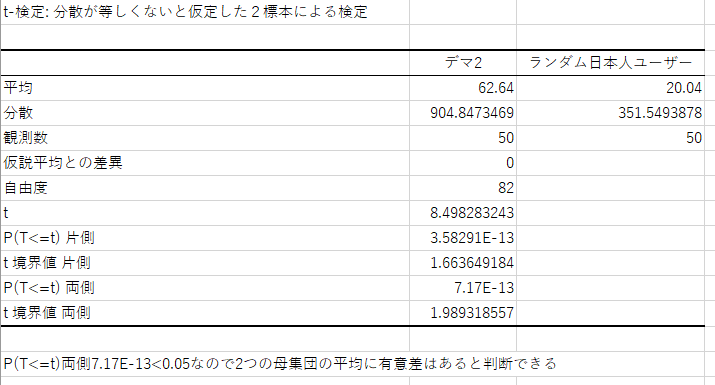
\includegraphics[width=13cm]{19.png}
\caption{t検定結果2}\label{31}
\end{figure}
\clearpage

\section{2標本t検定の結果3}
ランダムサンプリングした日本人ユーザー50人とデマツイート3をリツイートしたユーザー50人の最新100ツイートに含まれるリツイートの数で2標本t検定を行った結果を以下に示す.

\begin{figure}[htb]
\centering
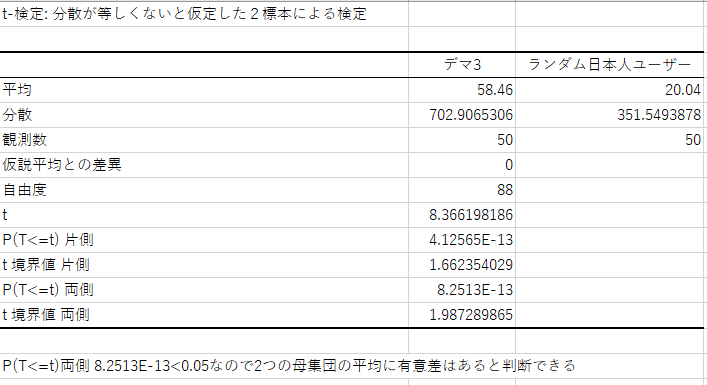
\includegraphics[width=13cm]{20.png}
\caption{t検定結果3}\label{32}
\end{figure}
\clearpage

\section{2標本t検定の結果4}
ランダムサンプリングした日本人ユーザー50人とデマツイート4をリツイートしたユーザー50人の最新100ツイートに含まれるリツイートの数で2標本t検定を行った結果を以下に示す.

\begin{figure}[htb]
\centering
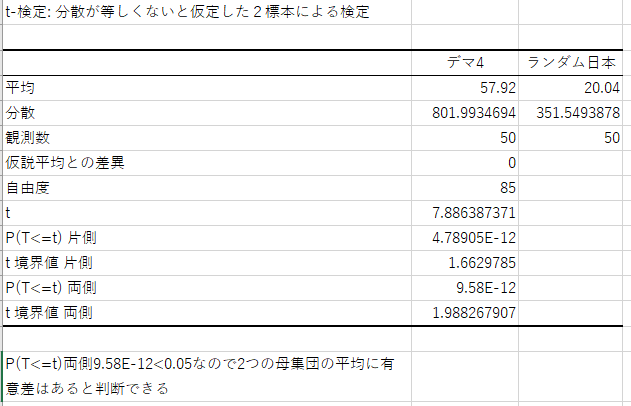
\includegraphics[width=13cm]{21.png}
\caption{t検定結果4}\label{33}
\end{figure}
\clearpage

\chapter{考察}
デマを拡散するようなユーザに共通する特徴として,リツイート数に着目しランダムサンプリングしたユーザーとデマツイートをリツイートしたユーザーで直近100リツイート内のリツイート数を調査した結果,大きく数値が異なった.この結果からデマを拡散するようなユーザーはリツイート機能を多用する傾向にあり,ツイート内容の真偽を確かめる前にリツイートをし,デマ拡散者の一員となっていると考えられる.

自分がデマ拡散者にならない為の手段として,デマ拡散ユーザーリストにあるユーザーと,リツイートの多いユーザーを排除することが有効だと考えられる.


\chapter{結論}
本研究では,デマが拡散されることを防ぐために,デマツイートをリツイートしているユーザーの特徴抽出としてリツイート数の調査を行った.その結果,デマツイートを拡散するユーザーの特徴として,ツイートに占めるリツイートの割合が高いことが確認できた.このような知識を活用することで,Twitterを閲覧する際に,デマツイートを真に受けて拡散してしまうリスクを下げられることが期待できる.


\bibliographystyle{junsrt}
\bibliography{biblio}%「biblio.bib」というファイルが必要.

\chapter*{謝辞}


本研究を進めるにあたり,矢吹研究室矢吹太朗准教授には,多くの時間をご指導にさいて頂きました.
また矢吹研究室の皆様には,多くの知識や示唆を頂きました.協力していただい皆様に感謝の気持ちと御礼を申し上げます.

\addcontentsline{toc}{chapter}{謝辞}

\end{document}
